\documentclass[11pt]{report}

\usepackage{fullpage}

\usepackage{common}
\usepackage{drawing}
\usepackage{tables}
\usepackage{notation}
\usepackage{linear}
\usepackage{probability}

% Set document meta data
\hypersetup{
    pdftitle = {Mathematics Notes},
    pdfauthor = {Brendan Burkhart}
}

\begin{document}

\begin{titlepage}
    \centering
    \vspace*{1cm}
	{\scshape\huge Mathematics Notes \par}
    \vspace{1cm}
    {\Large Foundations of mathematics and applications \par}
    \vfill
    \vfill
    \begin{tikzpicture}
        % define Lindenmayer system for tree
\pgfdeclarelindenmayersystem{Fractal tree}{
    \symbol{S}{\pgflsystemstep=0.625\pgflsystemstep} % Reduces size of sub-tree
    \rule{L->SF[++L][--L]} % Leaf becomes branch plus two leaves
}

% draw tree and clip to circle
\begin{scope}
    \clip (0, 1) circle (5);
    \filldraw[fill=black] (-5,0) rectangle (5,-5);

    \draw[rotate=90, line width=3pt] (-0.25, 0) [l-system={Fractal tree, step=2.25cm, angle=15, axiom=F[++++L][L][----L], order=6}] lindenmayer system -- cycle;
    \draw[rotate=-90, line width=2pt,draw=white] (0, 0) [l-system={Fractal tree, step=2cm, angle=15, axiom=[+++L][L][---L], order=4}] lindenmayer system -- cycle;
\end{scope}

% draw border circle
\draw[line width=3pt] (0, 1) circle (5);

    \end{tikzpicture}
    \vfill
    \vfill
    \vfill
    {\scshape\large Brendan Burkhart \par}
    \vspace{0.5cm}
    {\scshape Johns Hopkins University \par}
    \vfill
\end{titlepage}

\tableofcontents
\newpage

\parskip=1em
\parindent=0em

\documentclass[12pt]{article}

\usepackage{amsmath}
\usepackage{amssymb}
\usepackage{amsthm}
\usepackage{centernot}
\usepackage{fullpage}
\usepackage{makecell}
\usepackage{tabularx}
\usepackage[hypcap=false]{caption}
\usepackage{tikz}
\usepackage{titling}
\usepackage{pdfpages}
\usepackage{enumitem}
\usepackage{multicol}

\usepackage{common}

\begin{document}

\title{Discrete Mathematics}
\author{Brendan Burkhart}
\maketitle

\tableofcontents
\newpage

\section{Binomial Coefficients}

\begin{defn}\label{binomial-coefficient}
Let $n, k \in \N$. The \emph{binomial coefficient} $n \choose k$ is the number of subsets with cardinality $k$ of a set with cardinality $n$.
\end{defn}

\begin{exmp}\proofbreak
    \begin{multicols}{2}
        \begin{itemize}
            \item $\binom{0}{0} = 1$
            \item $\binom{1}{0} = 1$
            \item $\binom{1}{1} = 1$
            \item $\binom{2}{1} = 2$
            \item $\binom{3}{2} = 3$
            \item $\binom{4}{2} = 6$
        \end{itemize}

        \columnbreak

        \begin{itemize}
            \item $\binom{5}{0} = 1$
            \item $\binom{5}{1} = 5$
            \item $\binom{5}{2} = 10$
            \item $\binom{5}{3} = 10$
            \item $\binom{5}{4} = 5$
            \item $\binom{5}{5} = 1$
        \end{itemize}
    \end{multicols}
\end{exmp}

\begin{prop}\label{binomial-complement}
    Let $n, k \in \N$ with $0 \leq k \leq n$. Then \[{n \choose k} = {n \choose n-k}.\]
\end{prop}

\begin{proof}
    Any selection of $k$ elements from a set with $n$ elements is equivalent to the selection of the other $n-k$ elements.
\end{proof}

\begin{exmp}
    $\binom{5}{2} = \binom{5}{3}$, and $\binom{3}{1} = \binom{3}{2}$.
\end{exmp}

\begin{defn}\label{pascals-triangle}
    \emph{Pascal's Triangle} is a particular way of writing out what is essentially a table of binomial coefficients that highlights several properties. Rows represent successive values for $n$, and columns represent $k$ --- the first row contains only a single column where $k=0$, in the second row the columns are $k=0$ and $k=1$, and so on.
    \begin{center}
        \begin{tabular}{rccccccccc}
            $n=0$:&    &    &    &    &  1\\\noalign{\smallskip\smallskip}
            $n=1$:&    &    &    &  1 &    &  1\\\noalign{\smallskip\smallskip}
            $n=2$:&    &    &  1 &    &  2 &    &  1\\\noalign{\smallskip\smallskip}
            $n=3$:&    &  1 &    &  3 &    &  3 &    &  1\\\noalign{\smallskip\smallskip}
            $n=4$:&  1 &    &  4 &    &  6 &    &  4 &    &  1\\\noalign{\smallskip\smallskip}
        \end{tabular}
    \end{center}
\end{defn}

\begin{rmk}
    Notice that $\binom{n}{0} = \binom{n}{n} = 1$, since there is only one set with cardinality $0$ (the empty set), and the only subset with cardinality $n$ of a set $X$ itself with cardinality $n$ is $X$. Alternatively, since $\binom{n}{0} = 1$, by Proposition \ref{binomial-complement} it follows that $\binom{n}{0} = \binom{n}{n}$ and so $\binom{n}{n} = 1$.
\end{rmk}

\begin{rmk}
    Note that each entry in Pascal's Triangle is the sum of the two elements immediately above it.
\end{rmk}

\begin{prop}{Pascal's Identity}\label{pascals-identity}
    Let $n \in \N$ with $0 < k < n$. Then $\binom{n}{k} = \binom{n-1}{k-1} + \binom{n-1}{k}$.
\end{prop}

\begin{proof}
    Let $X$ be a set with $|X| = n$. By Definition \ref{binomial-coefficient}, $\binom{n}{k}$ is the number of subsets with $k$ elements of $X$. Fix some $x \in X$. Then there are $\binom{n-1}{k}$ subsets of $X$ that do not include $x$, and $\binom{n-1}{k-1}$ which do, so $\binom{n}{k} = \binom{n-1}{k-1} + \binom{n-1}{k}$.
\end{proof}

\begin{thm}{Binomial theorem}\label{binomial-theorem}\proofbreak
    Let $F$ be a field. Then for any $x, y \in F$ and $n \in \Z_{\geq 1}$, \[\left(x + y\right)^n = \sum_{k=0}^n x^ky^{n-k}{n \choose k}.\]
\end{thm}

\begin{proof}
    We will prove this by induction. Our base case is when $n = 1$, so $(x + y)^n = x + y$. Then \[\sum_k=0^1x^ky^{1-k}\binom{1}{k} = x^0y^1\binom{1}{0} + x^1y^0\binom{1}{1} = x + y,\] so the base case is true.
    Now assume that for some $x, y \in F$ and $n \geq 1$ we have \[\left(x + y\right)^n = \sum_{k=0}^n x^ky^{n-k}{n \choose k}.\] Then since $(x + y)^{n+1} = (x+y)(x+y)^n$, we have $(x = y)^{n+1} = x(x+y)^n + y(x+y)^n$.
    Therefore, \[\left(x + y\right)^{n+1} = x\left(\sum_{k=0}^n x^ky^{n-k}\binom{n}{k}\right) + y\left(\sum_{k=0}^n x^ky^{n-k}\binom{n}{k}\right),\] so it follows that \[\left(x + y\right)^{n+1} = \left(\sum_{k=0}^n x^{k+1}y^{n-k}\binom{n}{k}\right) + \left(\sum_{k=0}^n x^ky^{n-k+1}\binom{n}{k}\right).\]
    We can now re-index the left sum to make the form of the terms match up better: \[\left(x + y\right)^{n+1} = \left(\sum_{k=1}^{n+1} x^{k}y^{n-k+1}\binom{n}{k-1}\right) + \left(\sum_{k=0}^n x^ky^{n-k+1}\binom{n}{k}\right).\]
    Now we can factor and match up all the terms except for the last term of the left sum, and the first term of the right sum.
    \[\left(x + y\right)^{n+1} = y^{n+1}\binom{n}{0} + \left(\binom{n}{k-1} + \binom{n}{k}\right)\left(\sum_{k=0}^{n} x^{k}y^{n-k+1}\right) + x^{n+1}\binom{n}{n}.\]
    By Pascal's Identity \ref{pascals-identity}, we then have
    \[\left(x + y\right)^{n+1} = y^{n+1}\binom{n}{0} + \binom{n+1}{k}\left(\sum_{k=0}^{n} x^{k}y^{n-k+1}\right) + x^{n+1}\binom{n}{n}.\]
    We can then move the two extra terms into the summation:
    \[\left(x + y\right)^{n+1} = \sum_{k=0}^{n+1}x^{k}y^{n+1-k}\binom{n+1}{k}.\]
    Therefore, the induction step is complete, and so by the induction principle we are done.
\end{proof}

\begin{prop}
    Let $n, k \in \N$ with $0 \leq k \leq n$. Then \[\binom{n}{k} = \frac{n!}{k!(n-k)!}.\]
\end{prop}

\end{document}

\documentclass[12pt]{article}

\usepackage{amsmath}
\usepackage{amssymb}
\usepackage{amsthm}
\usepackage{fullpage}
\usepackage{makecell}
\usepackage{tabularx}
\usepackage[hypcap=false]{caption}
\usepackage{tikz}
\usepackage{titling}
\usepackage{pdfpages}
\usepackage{enumitem}

\usepackage{common}

\begin{document}

\title{Introduction to Analysis Notes}
\date{}
\author{Brendan Burkhart}
\maketitle

\tableofcontents
\newpage

\section{Sets and Lists}

\begin{defn}\label{set}
    A set is an unordered group of distinct elements.
\end{defn}

\begin{exmp}
    $\{1, 2, 3\}$ is a set containing three elements: $1$, $2$, and $3$.
\end{exmp}

\begin{note}
    $\{1, 2, 3, 3\}$ is also set containing three elements, since the elements of a set are distinct.
\end{note}

\begin{defn}\label{empty-set}
    The empty set (denoted $\emptyset$) is the unique set having no elements.
\end{defn}

One of the most fundamental operations of sets is the ``element of'' operation, denoted by $\in$. $x \in X$ is true precisely when $x$ is an element of the set $X$. Note that sets can be elements of other sets. $x \notin X$ is used to denote ``not an element of''.

\begin{exmp}
    $\left\{\{1, 2\}, \{\}\right\}$ is a set containing two elements: the set $\{1, 2\}$, and the empty set.
\end{exmp}

Set comprehensions, or set builder notation, is a method of precisely defining a set. It can take various forms, such as enumerating all (or implying such) the elements of a set (e.g. $\{1, 2\}$ or $\{1, 2, \ldots, 5\}$). Or it can be used to build a set from another, such as $\left\{2n \compbar n \in \N\right\}$, which says make a set by taking every natural number and doubling it --- these are, of course, the even natural numbers. Set comprehensions can be made more complicated by including a predicate, for example $\left\{n \in \N \compbar n \neq n^2 \right\}$ --- all natural numbers which are not their own square.

Two sets are equal when they contain precisely the same elements. For example, if we let $A = \{1, 1, 5, 2\}$ and $B = \{2, 2, 2, 1, 5\}$, then $A = B$ since for every element $x$ in $A$, $x$ is also in $B$ and vice versa.

\begin{defn}\label{subset}
    A set $T$ is a \emph{subset} of a set $S$ when every element of $T$ is also an element of $S$. This relationship is denoted $T \subseteq S$. $S$ is also referred to as a \emph{super set} of $T$.
\end{defn}

\begin{exmp}
    $\{1, 2, 3\}$ is a subset of $\{1, 2, 3\}$.
\end{exmp}

\begin{rmk}
    If a set $A$ is a subset of set $B$, and $B$ is a subset of $A$, then the sets must be equal. Showing that $A \subseteq B$ and $B \subseteq A$ is a common way to prove that two sets are equal.
\end{rmk}

\begin{defn}\label{proper-subset}
    A set $T$ is a \emph{proper subset} of a set $S$ when every element of $T$ is also an element of $S$, but not vice versa --- that is, the sets are not equal. This relationship is denoted $T \subset S$.
\end{defn}

\begin{exmp}
    $\{1\}$ is a proper subset of $\{1, 2, 3\}$.
\end{exmp}

\begin{defn}\label{intersection}
    The intersection of sets $A$ and $B$ is the set $\left\{x \compbar x \in A \land x \in B \right\}$. It is denoted by $A \intersection B$.
\end{defn}

\begin{exmp}
    $\{1, 2, 3, 4\} \intersection \{3, 4, 5\} = \{3, 4\}$.
\end{exmp}

\begin{defn}
    The union of sets $A$ and $B$ is the set $\left\{x \compbar x \in A \lor x \in B\right\}$. It is denoted by $A \union B$.
\end{defn}

\begin{exmp}
    $\{1, 2, 3, 4\} \union \{3, 4, 5\} = \{1, 2, 3, 4, 5\}$.
\end{exmp}

\begin{rmk}
    If $A$ and $B$ are sets, then $(A \intersection B) \subseteq (A \union B)$. $A = B$ if and only if $(A \intersection B) = (A \union B)$.
\end{rmk}

\begin{defn}
    The complement of set $A$ with respect to some super set $U$ is the set $\left\{x \in U \compbar x \notin A\right\}$. The complement is sometimes denoted $A'$.
\end{defn}

\begin{exmp}
    Let $U = \{1, 2, 3, 4, 5\}$, and $A = \{1, 2\}$. Then $A' = \{3, 4, 5\}$.
\end{exmp}

\begin{exmp}
    Let $U = \Z$, and $A$ the even numbers. Then $A'$ is the set of the odd numbers. 
\end{exmp}

\begin{rmk}
    $A' \union A = U$. $A' \intersection A = \emptyset$.
\end{rmk}

\begin{defn}\label{set-difference}
    The set difference of sets $A$ and  $B$, denoted $A \setminus B$, is the set containing all elements of $A$ which are not elements of $B$. $A \setminus B = \left\{x \in A \compbar x \notin B\right\}$.
\end{defn}

\begin{defn}\label{symmetric-difference}
    The symmetric difference of sets $A$ and $B$, denoted $A \triangle B$, is defined to be the set $(A \setminus B) \union (B \setminus A)$.
\end{defn}

\begin{rmk}
    $(A \triangle B)' = (A \intersection B)$ when $U = A \union B$.
\end{rmk}

While sets are unordered groups of distinct elements, lists (also called $n$-tuples) are ordered groups of elements which are not necessarily distinct. An ordered pair $(a, b)$ is a list of a length two (a tuple), where $a$, and $b$ are elements of some set.

\begin{defn}\label{tuple}
    An ordered pair $(a, b)$ is a tuple of elements of some set.
\end{defn}

Ordered pairs (and $n$-tuples more generally) can be represented as sets themselves --- the pair $(a, b)$ can be represented as the set $\left\{a, \{a, b\}\right\}$.

\begin{defn}\label{cartesian-product}
    The Cartesian product of two sets $A$ and $B$ is denoted $A \times B$. It is equal to $\left\{\left(a, b\right) \compbar a \in A, b \in B \right\}$.
\end{defn}

\section{Boolean Algebra}

Boolean algebra is the algebra dealing exclusively with the values \emph{true} and \emph{false}.

The primary operations of Boolean algebra are \emph{negation} (also called \emph{not}) denoted by $\neg$, \emph{conjunction} (also called \emph{and}) denoted by $\land$, and \emph{disjunction} (also called \emph{or}) denoted by $\lor$.

Since Boolean algebra has only two elements, it is possible to enumerate all variable combinations for a function. This is often done in the form of a truth table --- a table listing the values of variables and the corresponding function value as rows. For example, Table \ref{primary-operations} gives a combined truth table for negation, conjunction, and disjunction. It also serves as the definition of these operations.

\begin{center}
    \captionof{table}{Truth table of primary operations}
    \label{primary-operations}
    \begin{tabularx}{\linewidth}{|X|X|X|X|X|}
        \hline
        \thead{$X$} & \thead{$Y$} & \thead{$\neg X$} & \thead{$X \land Y$} & \thead{$X \lor Y$} \\
        \hline
        True  & True & False & True & True \\
        \hline
        True  & False & False & False & True \\
        \hline
        False  & True & True & False & True \\
        \hline
        False  & False & True & False & False \\
        \hline
    \end{tabularx}
\end{center}

\end{document}

\documentclass[12pt]{article}

\usepackage{amsmath}
\usepackage{amssymb}
\usepackage{amsthm}
\usepackage{fullpage}
\usepackage{makecell}
\usepackage{tabularx}
\usepackage{tikz}
\usepackage{titling}
\usepackage{pdfpages}
\usepackage{color}
\usepackage{hyperref}

\usepackage{common}
\usepackage{linear}

\begin{document}

\title{Linear Algebra Notes}
\author{Brendan Burkhart}
\maketitle

\tableofcontents
\newpage

\section{Row operations and echelon form}

\begin{defn}\label{linear-eq}
    A \emph{linear equation} is an equation of the form $a_1x_1 + a_2x_2 + \cdots + a_nx_n = b$
\end{defn}

\begin{defn}\label{linear-sys}
    A \emph{system of linear equations} (or \emph{linear system}) is a set of linear equations of the same variables (e.g. $x_1, x_2, \ldots, x_n$).
\end{defn}

\begin{defn}\label{linear-sys-solutions}
    The \emph{solution set} of a system of linear equations is the intersection of the solution set of each individual linear equation.
\end{defn}

Systems of linear equations can be represented via matrices, where each column is a specific variable, each row is a linear equation, and the entries are the coefficients. Augmentations represent the constant term (denoted $b$ in definition \ref{linear-eq}).

\begin{exmp}
    The linear system \[\begin{linsys}{3}
            x &+ &2y &- &z &= &-1 \\
            2x &+ &2y &+ &z &= &1 \\
            3x &+ &5y &- &2z &= &-1
        \end{linsys}\] can be represented by the augmented matrix below.
    \[\begin{amatrix}{3}
            1 &2 &-1 &-1 \\
            2 &2 &1 &1 \\
            3 &5 &-2 &-1
        \end{amatrix}\]
\end{exmp}

Row operations are certain operations on matrices or systems of linear equations which can be used to simply or otherwise transform the system, while leaving the solution set unchanged.

\begin{defn}\label{row-op}
    Row operations: \begin{enumerate}
        \item Swap two rows/equations
        \item Multiply a single row by a non-zero scalar
        \item Add a scalar multiple of one row to another
    \end{enumerate}
\end{defn}

\begin{thm}
    If a linear system is obtained from another by one of the row operations, then the two systems have the same set of solutions.
\end{thm}

\begin{proof}\proofbreak
    \begin{enumerate}
        \item As the intersection of sets is commutative, by Definition \ref{linear-sys-solutions}, the solution set of a linear system is unaffected by the order of the individual linear systems, therefore swapping rows/equations does not change the solution set.
        \item Since multiplying a single row by a non-zero scalar is equivalent to multiplying both sides of the represented equation by that scalar, the solution set is clearly left unchanged.
        \item Since adding a multiple of one row to another row is equivalent to adding equal quantities to both sides of the equation, no solutions are removed from the solution set. If the row $(sb_1 + a_1)x_1 + (sb_2 + a_2) + \cdots + (sb_n + a_n)x_n = sk_b + k_a$ is the result of adding $s$ times row $b_1x_1 + \cdots + b_nx_n = k_b$ to row $a_1x_1 + \cdots + a_nx_n = k_a$, then $(sb_1 + a_1)x_1 + (sb_2 + a_2) + \cdots + (sb_n + a_n)x_n = s(b_1x_1 + \cdots + b_nx_n) + k_a$  which implies that $a_1x_1 + \cdots + a_nx_n = k_a$, so no information was lost and the solution set remains the same.
    \end{enumerate}
\end{proof}

\begin{defn}
    A matrix in (row) \emph{echelon form} has all rows of zeroes at the bottom, and the leading term of each row is to the right of the row leading term above it.
\end{defn}

\begin{defn}
    In \emph{reduced row echelon form}, a matrix in row echelon form additionally has leading terms which are all $1$, and the entries above and below each leading term are zero.
\end{defn}

\begin{rmk}
    The reduced row echelon form of a particular matrix is always unique, however the row echelon form is not. Additionally, it is always possible to transform a given matrix into either echelon form via the row operations.
\end{rmk}

\begin{exmp}
    \begin{align*}
        \begin{amatrix}{3}
            1 &0 &1 &4 \\
            1 &-1 &2 &5 \\
            4 &-1 &5 &17
        \end{amatrix}
         & \begin{aligned}
             & \ro{r_2 \rightarrow r_2 - r_1}  \\
             & \ro{r_3 \rightarrow r_3 - 4r_1} \\
        \end{aligned}
         & \begin{amatrix}{3}
            1 &0 &1 &4 \\
            0 &-1 &1 &1 \\
            0 &-1 &1 &1
        \end{amatrix}
         & \begin{aligned}
             & \ro{r_2 \rightarrow -r_2} \\
        \end{aligned}
         & \begin{amatrix}{3}
            1 &0 &1 &4 \\
            0 &1 &-1 &-1 \\
            0 &-1 &1 &1
        \end{amatrix} \\
         & \begin{aligned}
             & \ro{r_3 \rightarrow r_3 + r_2} \\
        \end{aligned}
         & \begin{amatrix}{3}
            1 &0 &1 &4 \\
            0 &1 &-1 &-1 \\
            0 &0 &0 &0
        \end{amatrix}
    \end{align*}

    Since there is no leading term corresponding to $z$, $z$ is a free variable. If we let $z$ be zero, then the augmentation yields a particular solution to this linear system.

    Solution set in vector form:
    \[\begin{pmatrix}
            x \\ y \\ z
        \end{pmatrix} = \begin{pmatrix}
            4 \\ -1 \\ 0
        \end{pmatrix} + z\begin{pmatrix}
            -1 \\ 1 \\ 1
        \end{pmatrix}\]

    Solution set in parametric form:
    \[\left\{\left(4 - z, -1 + z, z\right) \compbar z \in \R \right\}\]

\end{exmp}

\section{Vector Spaces}

\begin{defn}
    Let $F$ be a field. A \emph{vector space} over $F$ consists of a set $V$ together with two operations:

    \begin{itemize}
        \item[] $+: V \times V \to V$ (vector addition)
        \item[] $\cdot: F \times V \to V$ (scalar multiplication)
    \end{itemize}
    which satisfy the following axioms for all $v, w, e \in V$ and $r, s \in F$:
    \begin{enumerate}
        \item $v + w = w + v$ (additive commutativity)
        \item $(v + w) + u = v + (w + u)$ (additive associativity)
        \item $\exists \vec{0} \in V \textrm{ s.t. } v + \vec{0} = v$ (additive identity)
        \item $\exists z \in V \textrm{ s.t. } v + z = \vec{0}$ (additive inverse)
        \item $(r + s) \cdot v = r \cdot v + s \cdot v$ (distributivity over scalar addition)
        \item $r \cdot (v + w) = r \cdot v + r \cdot w$ (distributivity over vector addition)
        \item $(rs)\cdot v = r \cdot (s \cdot v)$ (multiplicative associativity)
        \item $1 \cdot v = v$ (multiplicative identity)
    \end{enumerate}
\end{defn}

\begin{rmk}
    You can prove the following for all $v \in V$ and $r \in F$ from those axioms (see Lemma \ref{vector-space-properties}): 
    \begin{itemize}
        \item The additive identity ($\vec{0}$) is unique.
        \item Additive inverses are unique.
        \item $0 \cdot v = \vec{0}$.
        \item $-1 \cdot v = -v$.
        \item $r \cdot \vec{0} = \vec{0}$.
    \end{itemize}
\end{rmk}

\begin{exmp}
    $\R^n$ is a vector space over $\R$ with $+$ and $\cdot$ defined as usual.
\end{exmp}

\begin{exmp}
    Let $F$ be any field. Then \[F^n = \left\{\begin{pmatrix}
            x_1 \\ \vdots \\ x_n
        \end{pmatrix} \compbar x_i \in F \textrm{ for } i = 1, \ldots, n \right\}\] is a vector space over $F$ with $x + y$ defined as \[\begin{pmatrix}
            x_1 \\ \vdots \\ x_n
        \end{pmatrix} + \begin{pmatrix}
            y_1 \\ \vdots \\ y_n
        \end{pmatrix} = \begin{pmatrix}
            x_1 + y_1 \\ \vdots \\ x_n + y_n
        \end{pmatrix}\] and $r \cdot x$ defined as \[r\begin{pmatrix}
            x_1 \\ \vdots \\ x_n
        \end{pmatrix} = \begin{pmatrix}
            rx_1 \\ \vdots \\ rx_n
        \end{pmatrix}.\]
\end{exmp}

Consider the field $\mathbb{F}_2 = \{0, 1\}$, and the vector space $\mathbb{F}_2^2$. This vector space has four elements: $\left\{\begin{pmatrix}
        0 \\ 0
    \end{pmatrix}, \begin{pmatrix}
        0 \\ 1
    \end{pmatrix}, \begin{pmatrix}
        1 \\ 0
    \end{pmatrix}, \begin{pmatrix}
        1 \\ 1
    \end{pmatrix}\right\}$. In general, $\mathbb{F}_2^n$ has $2^n$ elements. Note that since $0 + 0 = 0$ and $1 + 1 = 0$, every element of $\mathbb{F}_2^n$ is its own inverse. Furthermore, every element of \textit{any} vector space $V$ over $\mathbb{F}_2$ is its own inverse. This is because $v + v = 1 \cdot v + 1 \cdot v = (1 + 1) \cdot v = 0 \cdot v = \vec{0}$.

Consider the empty set. It cannot be a vector space, since a vector space requires the existence of an additive identity. However, the set $V = \left\{\star\right\}$ with $\star \cdot \star = \star$ and $r \cdot \star = \star$ is a vector space, called the \textbf{trivial} vector space. Note that $\star = \vec{0}$.

\begin{exmp}
    $\C$ forms a vector space over $\R$, with element-wise addition and $r \cdot (a + bi) = (ra) + (rb)i$.
\end{exmp}

\begin{rmk}
    $\C =\C^1$ forms a vector space over $\C$, as does $\R = \R^1$ over $\R$.
\end{rmk}

\begin{exmp}
    Let $V$ be the set of $2 \times 2$ matrices over $\R$, denoted $M_{2 \times 2}(R)$:
    \[\left\{\begin{pmatrix}
            a & b \\ c & d
        \end{pmatrix} \compbar a,b,c,d \in \R \right\}.\] Define vector addition and scalar multiplication as follows. \[\begin{pmatrix}
            a & b \\ c &d
        \end{pmatrix} + \begin{pmatrix}
            a' & b' \\ c' &d'
        \end{pmatrix} = \begin{pmatrix}
            a + a' & b + b' \\ c + c' &d + d'
        \end{pmatrix}\] \[r \cdot \begin{pmatrix}
            a & b \\ c &d
        \end{pmatrix} = \begin{pmatrix}
            ra & rb \\ rc &rd
        \end{pmatrix}\] Note that $V$ is essentially equivalent to $\R^4$. $V$ is a vector space over $\R$, and in general $M_{m\times n}(F)$ with entry-wise vector addition and scalar multiplication forms a vector space over $F$.
\end{exmp}

\begin{exmp}
    Let $F$ be any field, and $n \in \N$. Then define the set $P_n(F)$, the set of all polynomials with coefficients in $F$ of degree at most $n$, as follows. \[P_n(F) = \left\{a_0 + a_1x_1 + \cdots + a_nx^n \compbar a_i \in F \textrm{ for }i=0,\ldots,n\right\}\] \[(a_0 + \cdots + a_nx^n) + (b_0 + \cdots + b_nx^n) = (a_0 + b_0) + \cdots + (a_n + b_n)x^n\] \[r(a_0 + \cdots + a_nx^n) = ra_0 + \cdots + ra_nx^n\]

    $P_n(F)$ is a vector space over $F$. Similarly, $P(F)$ (the set of polynomials with coefficients in $F$ of \textit{any} degree) forms a vector space over $F$.
\end{exmp}

\begin{exmp}
    Let $S$ be any set, $F$ any field, and $V = \{f: S \to F\}$. $V$ forms a vector space over $F$ with $(f + g)(s) = f(s) + g(s)$ and $(rf)(s) = r(f(s))$ for all $r \in F, s \in S$.
    
    Notice that if $S = \{1, \ldots, n\}$, we get $F^n$, since $f \in V$ is a function from a coordinate index $i$ to the value of that coordinate $x_i$. If $S = \N$ and $V = \left\{(a_1, a_2, \ldots) \compbar a_i \in F \textrm{ for } i = 1, 2, \ldots\right\}$, we similarly get the set of all sequences in $F$.
\end{exmp}

\begin{lemma}\label{vector-space-properties}
    Let $V$ be a vector space over a field $F$. Then for all $v \in V$ and $r \in F$: \begin{enumerate}
        \item The additive identity is unique.
        \item The additive inverse of $v$ is unique.
        \item $0 \cdot v = \vec{0}$.
        \item $(-1) \cdot v + v = \vec{0}$.
        \item $r \cdot \vec{0} = \vec{0}$.
    \end{enumerate}
\end{lemma}

\begin{proof}\proofbreak
    \begin{enumerate}
        \item Let $i_1$ and $i_2$ be additive identities of $V$. Then $i_1 = i_1 + i_2 = i_2$, and by transitivity $i_1 = i_2$. The additive identity is therefore unique.
        \item Let $w_1$ and $w_2$ be additive inverses of $v$. Then $v + w_1 = \vec{0}$ and $v + w_2 = \vec{0}$, so $v + w_1 = v + w_2$. Then $w_1 + (v + w_1) = w_1 + (v + w_2)$, which implies that $(w_1 + v) + w_1 = (w_1 + v) + w_2$. Therefore, $w_1 = w_2$, so the additive inverse of $v$ is unique and so can be denoted $-v$.
        \item $0 \cdot v + 0 \cdot v = (0 + 0) \cdot v = 0 \cdot v = 0 \cdot v + \vec{0}$. Since we have additive inverses, we have cancellation, so $0 \cdot v = \vec{0}$.
        \item $(-1) \cdot v + v = (-1) \cdot v + 1 \cdot v = (-1 + 1) \cdot v = 0 \cdot v = \vec{0}$.
        \item $r \cdot \vec{0} = r \cdot (v + -v) = r \cdot (1 + -1) \cdot v = (r \cdot 0)\cdot v = 0 \cdot v = \vec{0}$.
    \end{enumerate}
\end{proof}

\begin{defn}
    Let $V$ be a vector space over $F$, and $W \subseteq V$. We say $W$ is a \emph{subspace} of $V$ if it is itself a vector space over $F$ with the operations defined as for $V$.
\end{defn}

\begin{exmp}
    Let $W = \left\{\begin{pmatrix}
            x \\ y \\ z
        \end{pmatrix} \in \R^3 \compbar x + y + z = 0\right\}$. $W$ is a vector subspace over $\R$ with the operations inherited from $\R^3$. $W$ is a plane within $\R^3$, with normal $(1, 1, 1)$.
\end{exmp}

\begin{prop}\label{subspace-proof}
    A subset $W$ of $V$ is a subspace if and only if
    \begin{enumerate}
        \item $W$ is non-empty.
        \item $W$ is closed under vector addition.
        \item $W$ is closed under scalar multiplication.
    \end{enumerate}
\end{prop}

\begin{proof}\proofbreak
    ($\Longrightarrow$) If $W$ is a subspace, then by definition it is itself a vector space, so it must contain $\vec{0}$ and so it is non-empty. Additionally, (2) and (3) follow from the definition of binary operations.

    ($\Longleftarrow$) Since $W$ is a subset of $V$ with the same operations, all axioms of vector spaces follow except for the existence of the additive identity and additive inverses, and $W$ being closed under vector addition and scalar multiplication (as these are defined as binary operations for $V$ rather than $W$).

    (2) and (3) then guarantee that $W$ is closed under vector addition and scalar multiplication. Since $W$ is closed under scalar multiplication, we know that $(0 \cdot w) \in W$ for any $w \in W$. Since $0 \cdot w = \vec{0}$, we know that $\vec{0} \in W$ so $W$ has an additive identity. Similarly, since $(-1 \cdot w) \in W$ and $-1 \cdot w = -w$, every element in $W$ must have an additive inverse.
\end{proof}

\begin{exmp}
    Let $V = \R^3$, $W = \left\{\begin{pmatrix}
            x \\ y \\ z
        \end{pmatrix} \in \R^3 \compbar x + y + z = 1\right\}$. Then $W$ cannot be a subspace of $V$, as $\vec{0} \notin W$.
\end{exmp}

\begin{exmp}
    Let $V =\R^n$, and $W$ be the set of solutions to a homogeneous system of equations (every equation is equal to zero). Then $\{\vec{0}\}$ is a solution to the system of linear equations, and since every solution is equal to zero, the set of solutions is closed under addition and multiplication, so $W$ is a subspace of $V$.
\end{exmp}

\begin{exmp}
    If $V$ is any vector space over $F$, then both $\{\vec{0}\}$ and $V$ are subspaces of $V$.
\end{exmp}

\begin{defn}
    $\left\{\vec{0}\right\}$ is the \emph{trivial} subspace.
\end{defn}

\section{Linear Combinations and Spans}

\begin{defn}
    Let $V$ be a vector space over $F$, and $S \subseteq V$ with $S \neq \emptyset$. We say $v \in V$ is a \emph{linear combination} of vectors in $S$ if \[v = c_1s_1 + \cdots + c_nc_n \textrm{ for some } n >1, c_i \in F, s_i \in S \textrm{for i} = 1,\ldots,n\]
\end{defn}

\begin{exmp}
    In $\R^3$, $\begin{pmatrix}
            2 \\ 3 \\ 0
        \end{pmatrix} = 2\begin{pmatrix}
            1 \\ 0 \\ 0
        \end{pmatrix} + 3\begin{pmatrix}
            0 \\ 1 \\ 0
        \end{pmatrix}$, so $\begin{pmatrix}
            2 \\ 3 \\ 0
        \end{pmatrix}$ is a linear combination of vectors in $\left\{\begin{pmatrix}
            1 \\ 0 \\ 0
        \end{pmatrix},\begin{pmatrix}
            0 \\ 1 \\ 0
        \end{pmatrix},\begin{pmatrix}
            0 \\ 0 \\ 1
        \end{pmatrix}\right\}$.
\end{exmp}

\begin{defn}
    Let $S \subseteq V$. The \emph{span} (also \emph{linear span} or \emph{linear hull}) of $S$ is the set of all linear combinations of vectors in $S$. \[\spanset{S} = \left\{c_1s_1 + \cdots + c_ns_n \compbar n \in \N, c_i \in F, s_i \in S\right\}\]

    By convention, if $S = \emptyset$, we define $\spanset{S} = \vec{0}$.
\end{defn}

\begin{rmk}
    If $S \subseteq T$, then $\spanset{S} \subseteq \spanset{T}$.
\end{rmk}

\begin{lemma}
    Let $V$ be a vector space over $F$, and $s \subseteq V$. Then $\spanset{S}$ is a subspace of $V$.
\end{lemma}

\begin{proof}
    If $S = \emptyset$, then $\spanset{S} = \left\{\vec{0}\right\}$, so $\spanset{S}$ is the trivial subspace.

    If $S \neq \emptyset$, then there exists some $s \in S$. Since $(1 \cdot s) \in \spanset{S}$, we know that $\spanset{S} \neq \emptyset$. Let $v, w \in \spanset{S}$, $r \in F$. We need to prove that $v + r \cdot w \in \spanset{S}$. Since $v \in \spanset{S}$, we know that $v = c_1s_1 + \cdots + c_ns_n$ for some $n \geq 1$, $c_i \in F$, and $s_i \in S$. Similarly, $w = d_1t_1 + \cdots + d_mt_m$ for some $m \geq 1$, $d_i \in F$, and $t_i \in S$. Then $v + rw = c_1s_1 + \cdots + c_ns_n + rd_1t_1 + \cdots + rd_mt_m$, so $v + r \cdot w \in \spanset{S}$. Therefore, by Lemma \ref{subspace-proof}, $\spanset{S}$ is a subspace of $V$.
\end{proof}

\begin{rmk}
    We also proved that $S \subseteq \spanset{S}$, and that $\spanset{S}$ is the smallest subspace of $V$ that contains $S$, in the sense that if $W$ is a subspace of $V$ such that $S \subseteq W$, then $\spanset{S} \subseteq W$.
\end{rmk}

\begin{exmp}
    Let $v$ be a vector space over $F$. Given $S \subseteq V$, and $v \in V$, how do we know if $v \in \spanset S$?

    Let $V = P_2(\R)$, $S = \left\{x^2 + 3x - 2, 2x^2 + 5x -3\right\}$, and $v = -x^2 - 4x + 4$. We are trying to determine $a, b \in F$ such that $-x^2 - 4x + 4 = a(x^2 + 3x - 2) + b(2x^2 + 5x - 3)$. This would imply that $a + 2b = -1$, $3a + 5b = -4$, and $-2a - 3b = 4$. This system of equations can be represented as a matrix, and solved for $a$ and $b$.
    \begin{align*}
        \begin{amatrix}{2}
            1 &2 &-1 \\
            3 &5 &-4 \\
            -2 &-3 &4
        \end{amatrix}
         & \begin{aligned}
             & \ro{r_2 \rightarrow r_2 - 3r_1}  \\
             & \ro{r_3 \rightarrow r_3 + 2r_1} \\
        \end{aligned}
         & \begin{amatrix}{2}
            1 &2 &-1 \\
            0 &-1 &-1 \\
            0 &1 &2
        \end{amatrix}
    \end{align*}
    This would imply that $0b = 1$, which is a contradiction, so no such $a, b$ exist.
\end{exmp}

\begin{lemma}
    Let $V$ be a vector space over $F$, $S \subseteq V$, and $v \in V$. Then $\spanset{S \cup \left\{v\right\}} = \spanset{S}$ if and only if $v \in \spanset{S}$.
\end{lemma}

\begin{proof}\proofbreak
    ($\Longrightarrow$) If $v \notin \spanset{S}$, then since $v \in \spanset{S \cup \left\{v\right\}}$, we know that $\spanset{S} \neq \spanset{S \cup \left\{v\right\}}$.

    ($\Longleftarrow$) Assume $v \in \spanset{S}$. Then $v = c_1v_1 + \cdots + c_ns_n$ for $c_i \in F$ and $s_i \in S$. Since $S \subseteq S \cup \left\{v\right\}$, we have $\spanset{S} \subseteq \spanset{S \cup \left\{v\right\}}$. Let $w \in \spanset{S \cup \left\{v\right\}}$, so $w = d_1t_1 + \cdots + d_mt_n + d_{m+1}v$. Thus, $w = d_1t_1 + \cdots + d_mt_m + d_{m+1}(c_1 + \cdots + c_n)$, so $w \in \spanset{S}$ and $\spanset{S \cup \left\{v\right\}} \subseteq \spanset{S}$. Therefore, $\spanset{S} = \spanset{S \cup \left\{v\right\}}$.
\end{proof}

\end{document}

\input{groups}
\documentclass[12pt]{article}

\usepackage{amsmath}
\usepackage{amssymb}
\usepackage{amsthm}
\usepackage{centernot}
\usepackage{fullpage}
\usepackage{makecell}
\usepackage{tabularx}
\usepackage[hypcap=false]{caption}
\usepackage{tikz, tkz-euclide}
\usetikzlibrary{decorations.pathreplacing,arrows}
\usetikzlibrary{quotes,angles,calc,intersections}

\usepackage{titling}
\usepackage{pdfpages}
\usepackage{enumitem}
\usepackage{multicol}
\usepackage{bm}

\usepackage{linear}
\usepackage{common}

\begin{document}

\title{Ordinary Differential Equations}
\author{Brendan Burkhart}
\maketitle

\tableofcontents
\newpage

\section{Classification}

\begin{defn}
    A \emph{differential equation} is an equation relating one or more independent variables, functions of those variables, and derivatives of those functions.
\end{defn}

\begin{exmp}\label{first-order-ode}
    \[\frac{\mathrm{d}x}{\mathrm{d}t} = x\]
\end{exmp}

\begin{defn}
    A \emph{solution} to a differential equation is an expression for the dependent functions of the differential equation in terms of the independent variables.
\end{defn}

Differential equations can be broadly classified into \emph{ordinary} and \emph{partial} differential equations.

\begin{defn}
    An \emph{ordinary} differential equation, or \emph{ODE} is a differential equation involving a single independent variable, and all derivatives are with respect to this variable.
\end{defn}

\begin{defn}
    A \emph{partial} differential equation, or \emph{PDE} is a differential equation involving functions of more than one independent variables, and derivatives may be with respect to any of those variables.
\end{defn}

\begin{defn}
    The \emph{general form} of an ODE is
    \[F(x, y, y', \ldots, y^{(n)}) = 0,\] that is some expression involving the independent variable $x$, the dependent variable $y$, and the derivatives of $y$.
\end{defn}

\begin{defn}
    The \emph{order} of a differential equation is the order of the highest derivative.
\end{defn}

\begin{exmp}
    \[\frac{\mathrm{d}^2\theta}{\mathrm{d}t^2} + \frac{g}{L}\sin\theta = 0\]
    This is a second order differential equation, while Example \ref{first-order-ode} is first order.
\end{exmp}

\begin{defn}
    A differential equation of a dependent variable $y$ and its derivatives is said to be \emph{linear} if it is an affine map with regard to $y$ and its derivatives.
\end{defn}

\begin{exmp}
    $\sin(x)y' + 2x^2y'' = x$ is linear.
\end{exmp}

\begin{exmp}
    $yy' + y'' = 0$ is non-linear.
\end{exmp}

\begin{defn}
    An \emph{autonomous} differential equation is one in which the independent variable does not explicitly appear. When the independent variable represents time in some way, these may also be called \emph{time-invariant}.
\end{defn}

\begin{exmp}
    $\frac{\mathrm{d}y}{\mathrm{d}x} = 5y - 20$ is an autonomous differential equation as the independent variable $x$ is not explicitly present.
\end{exmp}

\section{First-order linear autonomous differential equations}

Any first-order linear autonomous differential equation with independent variable $x$ and dependent variable $y$ can trivially be put into the form \[\frac{\mathrm{d}y}{\mathrm{d}x} = ay - b.\] This form can always be solved.

\begin{align*}
    \frac{\mathrm{d}y}{\mathrm{d}x} &= ay - b \\
    &= a(y - \frac{b}{a})
\end{align*}

Note that $\frac{\mathrm{d}}{\mathrm{d}x}{y - \frac{b}{a}} = \frac{\mathrm{d}}{\mathrm{d}x}y$. If $y \neq \frac{b}{a}$, it follows that $\ln(y - \frac{b}{a}) = ax + C$ for some constant of integration $C$, so $\abs{y - \frac{b}{a}} = ke^{ax}$ for some $k$. If $y > \frac{b}{a}$, then $y = \frac{b}{a} + ke^{ax}$, and similarly if $y < \frac{b}{a}$, then $y = \frac{b}{a} + ke^{ax}$ for some $k$. In the case that $y = \frac{b}{a}$, it follows that $\frac{\mathrm{d}y}{\mathrm{d}x} = 0$, so $y = \frac{b}{a} + ke^{ax}$ where $k = 0$.

Therefore, $y = \frac{b}{a} + ke^{ax}$ is a solution to any first-order linear autonomous differential equation.

\end{document}

\setchaptergraphic{
    % Hyperboloid of one sheet
    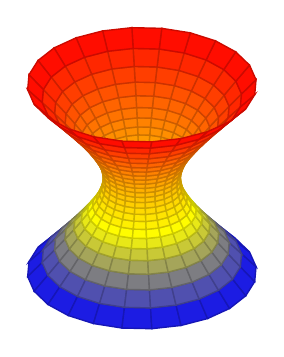
\begin{tikzpicture}[scale=1.25]
        \begin{axis}[hide axis,axis equal,colormap/hot]
            \addplot3[surf,domain=0:360,y domain=-1.75:1.75] ({cosh(y)*cos(x)},{cosh(y)*sin(x)},{sinh(y)});
        \end{axis}
    \end{tikzpicture}
    \hspace{1cm}
    % Saddle
    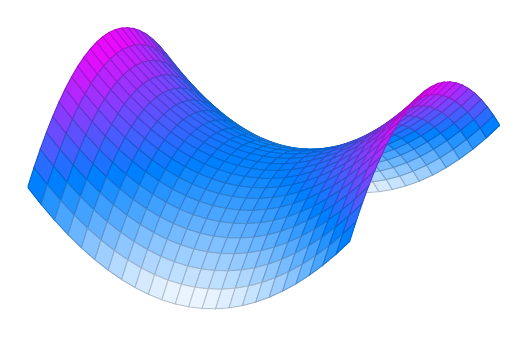
\begin{tikzpicture}[scale=0.875]
        \begin{axis}[hide axis,colormap/cool]
            \addplot3[surf,domain=-1.5:1.5,y domain=-1.5:1.5] {x^2-y^2};
        \end{axis}
    \end{tikzpicture}
}

\chapter{Vector Calculus}
\label{ch:vector-calc}

\section{Orthogonal Projection}

\begin{thm}\label{law-of-cosines}
    Let $\theta$ be the angle between non-zero vectors $A$ and $B$, and let $C = A - B$. The \emph{Law of Cosines} states that $\norm{C}^2 = \norm{A}^2 + \norm{B}^2 - 2\norm{A}\norm{B}\cos(\theta)$.
\end{thm}

\begin{figure}[ht!]
    \centering
    \begin{tikzpicture}[scale=1.4]
        \coordinate (O) at (0, 0);
        \coordinate (A) at (3, 5);
        \coordinate (B) at (6, 2);
        \coordinate (A') at ($(O)!(A)!(B)$);

        \draw [thick, ->] (O) -- (A);
        \draw [thick, ->] (O) -- (B);
        \draw [thick, dashed] (A') -- (A);
        \draw [very thick, red, ->] (O) -- (A');

        \draw [decorate,decoration={brace,amplitude=6pt,raise=3pt]}]
            (O) -- (A) node [black,midway,xshift=-0.6cm,yshift=0.3cm]
            {\footnotesize $A$};

        \draw [decorate,decoration={brace,amplitude=6pt,raise=3pt]}]
            (B) -- (O) node [black,midway,xshift=0.2cm,yshift=-0.5cm]
            {\footnotesize $B$};

        \draw [decorate,decoration={brace,amplitude=6pt,raise=3pt]}]
            (A) -- (A') node [black,midway,xshift=1.0cm, yshift=0.1cm]
            {\footnotesize $A - A'$};

        \draw [decorate,decoration={brace,amplitude=6pt,raise=3pt]}]
            (O) -- (A') node [black,midway,xshift=-0.2cm, yshift=0.5cm]
            {\footnotesize $A'$};

        \tkzMarkAngle[size=1cm,mark=|](B,O,A)
        \tkzLabelAngle[pos=1.2](B,O,A) {$\theta$}

        \tkzMarkRightAngle[size=0.4](A,A',O)
    \end{tikzpicture}
\caption{Orthogonal projection of $\vec{A}$ onto $\vec{B}$}
\label{fig:orthogonal-projection}
\end{figure}

Figure \ref{fig:orthogonal-projection} shows $A'$, the orthogonal projection of vector $A$ onto $B$. $\norm{A'}$ is the shortest distance between the head of $A$ and $B$.

\begin{thm}
    Let $\theta$ be the angle between non-zero vectors $A$ and $B$. Then $\cos\theta = \frac{A \cdot B}{\norm{A}\norm{B}}$.
\end{thm}

\begin{proof}\label{vector-angle}
    Let $C = A - B$. Then $C \cdot C = (A - B) \cdot (A - B)$, which can we expand to get $A \cdot (A - B) - B \cdot (A - B) = A \cdot A + B \cdot B - 2(A \cdot B)$. Therefore, $\norm{C}^2 = \norm{A}^2 + \norm{B}^2 - 2(A \cdot B)$. By the Law of Cosines \ref{law-of-cosines} and transitivity, it follows that $A \cdot B = \norm{A}\norm{B}\cos\theta$, so $\cos\theta = \frac{A \cdot B}{\norm{A}\norm{B}}$.
\end{proof}

\begin{exmp}
    Let $A = \left(0, 1\right)$, and $B = \left(2, 2\right)$. Then $\cos\theta = \frac{A \cdot B}{\norm{A}\norm{B}}$. Since $A \cdot B = 0 \cdot 2 + 1 \cdot 2 = 2$, $\norm{A} = \sqrt{0^2 + 1^2} = 1$, and $\norm{B} = \sqrt{2^2 + 2^2} = \sqrt{8} = 2\sqrt{2}$, we have $\cos\theta = \frac{2}{1 \cdot 2\sqrt{2}}$. This is equal to $\frac{\sqrt{2}}{2}$, so $\theta = \frac{\pi}{4}$.
\end{exmp}

\begin{exmp}
    Let $A = {1, 1}$ and $B = {1, -1}$. Then since $A \cdot B = 1 - 1 = 0$, we know $\cos\theta = 0$, which implies that $\theta = \frac{\pi}{2}$.
\end{exmp}

\begin{cor}\label{orthogonal-vectors}
    Non-zero $A$ and $B$ are orthogonal if and only if $A \cdot B = 0$.
\end{cor}

\begin{proof}
    Let $A$ and $B$ be non-zero orthogonal vectors. Then the angle ($\theta$) between $A$ and $B$ must be $\frac{\pi}{2}$ since they are orthogonal. By Theorem \ref{vector-angle}, $\cos\theta = \frac{A \cdot B}{\norm{A}\norm{B}}$. Since $A$ and $B$ are non-zero, $\norm{A}\norm{B}$ is non-zero, and since $\theta = \frac{\pi}{2}$, we know $\cos\theta = 0$. Therefore, $A \cdot B$ must equal zero.
\end{proof}

\begin{thm}\label{vector-projection}
    Let $A$ and $B$ be vectors, and $A'$ be the orthogonal projection of $A$ onto $B$. Then $A' = \frac{A \cdot B}{B \cdot B}B$.
\end{thm}

\begin{proof}
    Let $d \in \R$ such that $C = dB$. Then since $(A - dB) \cdot B = 0$, we know $A \cdot B - dB \cdot B = 0$, so $A \cdot B = d(B \cdot B)$. This implies that $d = \frac{A \cdot B}{B \cdot B}$. Since $C = dB$, we then have $C = \frac{A \cdot B}{B \cdot B}B$.
\end{proof}

\begin{exmp}
   Let $A = \left(2, 2\right)$, and $B = \left(1, 0\right)$. Then since $A \cdot B = 2$, and $B \cdot B = 1$, we know $A' = \frac{2}{1}B = \left(2, 0\right)$.
\end{exmp}

\begin{thm}
    Let $p$ be a point, and $A\cdot\vec{x} + D = 0$ be a plane. Then the distance from the point to the plane is given by $\frac{A\cdot p + D}{\norm{A}}$.
\end{thm}

\begin{proof}
    The line with direction $A$ that passes through $p$ is normal to the plane and thus contains the shortest path from the point to the plane. Therefore, $A \cdot (p + tA) + D = 0$ gives the closest point on the plane to $p$. We then have $A \cdot p + D = -t(A \cdot A)$. Since the shortest distance is equal to $|-t\norm{A}|$, it follows that the shortest distance is given by \[\frac{\abs{A \cdot p + D}}{\norm{A}}.\]
\end{proof}

\begin{cor}
    Let $(x_1, y_1, z_1)$ be a point in $\R^3$, and $Ax + By + Cz + D = 0$ be a plane in $\R^3$. Then the distance from the point to the plane is: \[\frac{\abs{Ax_1 + By_1 + Cz_1 + D}}{\sqrt{A^2 + B^2 + C^2}}.\]
\end{cor}

\section{Cross Product}

\begin{defn}
    The \emph{cross product} or \emph{vector product} of three-dimensional vectors $A = a_1i + a_2j + a_3k$ and $B = b_1i + b_2j + b_3k$ is written $A \times B$. \[A \times B = \begin{vmatrix}
        i & j & k \\ a_1 & a_2 & a_3 \\ b_1 & b_2 & b_3
    \end{vmatrix}\] The value of this determinant can be found via the Laplace formula (also called cofactor expansion) along any column or row. Expansion along the first row gives: \[A \times B =
    \begin{vmatrix}
        i & j & k \\ a_1 & a_2 & a_3 \\ b_1 & b_2 & b_3
    \end{vmatrix} =
    \begin{vmatrix}
        a_2 & a_3 \\ b_2 & b_3
    \end{vmatrix}i -
    \begin{vmatrix}
        a_1 & a_3 \\ b_1 & b_3
    \end{vmatrix}j +
    \begin{vmatrix}
        a_1 & a_2 \\ b_1 & b_2
    \end{vmatrix}k\] \[= (a_2b_3 - b_2a_3)i - (a_1b_3 - b_1a_3)j + (a_1b_2 - b_1a_2)k.\]
\end{defn}

\begin{rmk}
    The cross product is a non-commutative binary operation.
\end{rmk}

\begin{exmp}
    Let $A = 3i + j - k$, and $B = -6i - 2j - 2k$. Then \[A \times B =
    \begin{vmatrix}
        i & j & k \\ 3 & 1 & -1 \\ -6 & -2 & -2
    \end{vmatrix} = (-2 - 2)i - (-6 - 6)j + (-6 + 6)k = -4i + 12j + 0k.\]
\end{exmp}

\begin{thm}
    Let $A = a_1i + a_2j + a_3k$ and $B = b_1i + b_2j + b_3k$ be vectors. Then $A \times B$ is orthogonal to both $A$ and $B$.
\end{thm}

\begin{proof}
    Since $A \times B = (a_2b_3 - b_2a_3)i - (a_1b_3 - b_1a_3)j + (a_1b_2 - b_1a_2)k$, we know that $A \cdot (A \times B) = (a_1a_2b_3 - a_1b_2a_3) - (a_1a_2b_3 - b_1a_2a_3) + (a_1b_2a_3 - b_1a_2a_3)$. This is equal to $(a_1a_2b_3 - a_1a_2b_3) - (b_1a_2a_3 - b_1a_2a_3) + (a_1b_2a_3 - a_1b_2a_3)$, which is equal to $0$, so by Corollary \ref{orthogonal-vectors} we know $A$ is orthogonal to $A \times B$. Similarly, $B$ is orthogonal to $A \times B$.
\end{proof}

\begin{thm}
    Let $A$, $B$, and $C$ be vectors, and $x$ a real number. Then:
    \begin{itemize}
        \item $A \times B = \vec{0}$ if and only if $A = \vec{0}$, $B = \vec{0}$, or $A$ is parallel to $B$.
        \item $A \times B = -(B \times A)$.
        \item $A \times (B + C) = (A \times B) + (A \times C)$.
        \item $(A + B) \times C = (A \times C) + (B \times C)$.
        \item $(\alpha A) \times B = A \times (\alpha B) = \alpha(A \times B)$.
    \end{itemize}
\end{thm}

\begin{rmk}
    In a \emph{right-handed} coordinate system, the cross product will follow the \emph{right-hand rule}: on the right hand, index finger represents $A$, middle finger represents $B$, and then thumb represents $A \times B$. However, in a \emph{left-handed} coordinate system, the cross product will instead follow the similar \emph{left-hand rule}. The chirality of the cross product follows the chirality of the chosen basis, and is not inherently due to the definition of the cross product.
\end{rmk}

\begin{thm}
    Let $A$ and $B$ be two vectors, and $\theta$ be the angle between them. Then $\norm{A \times B} = \norm{A}\norm{B}\sin\theta$, which is the area of a parallelogram with side lengths $\norm{A}$ and $\norm{B}$ and angle $\theta$.
\end{thm}

\begin{thm}
    The shortest distance between two non-parallel lines $p_1 + t_1d_1$ and $p_2 + t_2d_2$ is given by \[\frac{(p_1 - p_2) \cdot (d_1 \times d_2)}{\norm{d_1 \times d_2}}.\]
\end{thm}

\begin{proof}
    The shortest distance must lay on a vector that is orthogonal to both lines, which would be $d_1 \times d_2$. The component of $p_1 - p_2$ onto $d_1 \times d_2$ is then the shortest distance between the lines.
\end{proof}

\begin{thm}
    The closest point on a line $p_1 + t_1d_1$ to another lines $p_2 + t_2d_2$ is \[p_1 + \frac{(p_2 - p_1)\cdot n}{d_1 \cdot n}d_1.\]
\end{thm}

\begin{proof}
    The vector between the closest point and $p_2$ must be parallel to $d_1 \times d_2$, so it will intersect the plane with normal $(d_1 \times d_2) \times d_2$. Let $n = (d_1 \times d_2) \times d_2$. Then \[\left\{(p_1 + t_1d_1) - p_2\right\} \cdot n = 0,\] so $(p_2 - p_1)\cdot n = t(d_1 \cdot n)$. Therefore, the closest point is given by \[p_1 + \left(\frac{(p_2 - p_1)\cdot n}{d_1 \cdot n}\right)d_1.\]
\end{proof}

\section{Alternative Coordinate Systems}

There are many useful alternatives to the Cartesian coordinate system, such as the polar, cylindrical, and spherical coordinate systems.

In polar coordinates, two-dimensional points are represented by a radius $r$ and an angle $\theta$. The $r$ is the radius from the origin, and $\theta$ is the angle measured anticlockwise around the origin, starting from the positive half of the $x$-axis.

\begin{thm}
    Let $(x, y)$ be a point in Cartesian coordinates. Then $(r, \theta)$, where
    \begin{itemize}
        \item $r = \sqrt{x^2 + y^2}$
        \item $\theta = \arctan\frac{y}{x}$
    \end{itemize} gives the same point in polar coordinates.
\end{thm}

\begin{thm}
    Let $(r, \theta)$ be a point in polar coordinates. Then $(x, y)$, where
    \begin{itemize}
        \item $x = r\cos\theta$
        \item $y = r\sin\theta$
    \end{itemize} gives the same point in Cartesian coordinates.
\end{thm}

\begin{exmp}
    $(2, 2)$ in Cartesian coordinates is $(\sqrt{4 + 4}, \arctan(\frac{2}{2})) = (2\sqrt{2}, \frac{\pi}{4})$ in polar coordinates.
\end{exmp}

Since $(r, \theta + 2\pi{n})$ and $(-r, \theta + 2\pi{n})$ represent the same point in polar coordinates for all $n \in \Z$, it is common to choose ranges for $r$ and $\theta$ to make the representation of any given point unique. One such scheme is to restrict $\theta$ to $\left[0, 2\pi\right)$, and $r > 0$ except for the unique origin, $(0, 0)$.

While the two-dimensional Cartesian coordinate system is extended to three dimensions by adding the $z$-axis, there are two different ways to extend the polar coordinate system to three dimensions: cylindrical and spherical coordinates.

In cylindrical coordinates, polar coordinates are augmented with a $z$-axis, so points are represented as $(r, \theta, z)$. The radius, $r$, is still measured within the $xy$ plane.

Let $(x, y, z)$ be a point in the Cartesian coordinate system, and $(r, \theta, z)$ be the same point in cylindrical coordinates. Then all the same relationships are true as for polar coordinates, with the addition that $z = z$.

\begin{exmp}
    $(2, 2, 5)$ in Cartesian coordinates is $(\sqrt{4 + 4}, \arctan(\frac{2}{2}), 5) = (2\sqrt{2}, \frac{\pi}{4}, 5)$ in cylindrical coordinates.
\end{exmp}

In spherical coordinates, polar coordinates are augmented with a zenith angle $\phi$, measured from the zenith ($z$-axis) down to the point. The radius is measured in three dimensions rather than just in the $xy$-plane, so it is typically represented using the symbol $\rho$ rather than $r$ to differentiate it from the polar radius.

\begin{thm}
    Let $(x, y, z)$ be a point in Cartesian coordinates. Then $(\rho, \theta, \phi)$, where
    \begin{itemize}
        \item $\rho = \sqrt{x^2 + y^2 + z^2}$
        \item $\theta = \arctan\frac{y}{x}$
        \item $\phi = \arccos\frac{z}{\rho}$
    \end{itemize} gives the same point in spherical coordinates.
\end{thm}

\begin{thm}
    Let $(\rho, \theta, \phi)$ be a point in spherical coordinates. Then $(x, y, z)$, where
    \begin{itemize}
        \item $r = \rho\sin\phi$
        \item $x = r\cos\theta$
        \item $y = r\sin\theta$
        \item $z = \rho\cos\phi$
    \end{itemize} gives the same point in Cartesian coordinates.
\end{thm}

\begin{exmp}
    If $(\sqrt{6}, -\sqrt{2}, -2\sqrt{2})$ is a point in Cartesian coordinates, then $\rho$ is equal to $\sqrt{6 + 2 + 8} = 4$, $\theta = \arctan\frac{-\sqrt{2}}{\sqrt{6}} = \frac{11\pi}{6}$, and $\phi = \arccos\frac{-2\sqrt{2}}{4} = \frac{3\pi}{4}$.
\end{exmp}

\section{Gradient}

\begin{defn}
    Let $f: \R^n \to \R$. Then the \emph{gradient} of $f$, denoted by $\nabla f$, is a vector representing the derivative of the function: \[\left\langle \frac{\partial f}{\partial x_1}, \frac{\partial f}{\partial x_2}, \ldots, \frac{\partial f}{\partial x_n} \right\rangle.\]
\end{defn}

\begin{defn}
    The \emph{directional derivative} of a function $f: \R^n \to \R$ in the direction given by a unit vector $v$ is $\nabla f \cdot v$.
\end{defn}

\begin{thm}
    The gradient of a function $f: \R^n \to \R$ is the direction that maximizes change.
\end{thm}

\begin{proof}
    Since $x \cdot y = \norm{x}\norm{y}\cos(\theta)$, it follows that the unit vector to maximizes the directional derivative is $\frac{\nabla f}{\norm{\nabla f}}$, as this is when $\cos(\theta)$ is maximized.
\end{proof}

\section{Surfaces}

\begin{defn}
    A \emph{level set} of a real-valued function for a value $c \in \R$ is the set of all points where the value of the function is $c$. For a function $f$ of $n$ real variables, the level set is \[L_c(f) = \left\{\left(x_1, x_2, \ldots, x_n\right) \compbar f(x_1, x_2, \ldots, x_n) = c\right\}.\]
\end{defn}

\begin{rmk}
    When $n = 2$, the level sets are called \emph{level curves}. These as essentially the same as contour lines on a topographical map. When $n=3$, the level sets are called \emph{level surfaces}.
\end{rmk}

\begin{prop}
    The tangent vector to a level set at a specific point is orthogonal to the gradient at that point.
\end{prop}

\begin{proof}
    Since the value of all points in a level set are equal, the directional derivative in the direction of a tangent to a level set must be zero. Let $v$ be a tangent vector at a point $p$. Then $\nabla f(p) \cdot \frac{v}{\norm{v}} = 0$ implies that $\nabla f(p)$ is orthogonal to $v$ by Corollary \ref{orthogonal-vectors}.
\end{proof}

\begin{defn}
    A \emph{cylinder} is a surface that consists of parallel lines that intersect a given plane curve. For a cylinder in the more typical sense, the plane curve is a circle.
\end{defn}

\begin{defn}
    \emph{Quadric surfaces} are higher-dimensional generalizations of conic sections --- ellipses, parabolas, and hyperbolas. In three dimensions with coordinate variables $x, y, z$, quadric surfaces are given by $Ax^2 + By^2 + Cz^2 + Dxy + Exz + Fyz + Gx + Hy + Iz + J = 0$.
\end{defn}

\begin{defn}
    An \emph{ellipsoid} with width ($x$) $a$, height ($y$) $b$, and depth ($z$) $c$ is \[\frac{x^2}{a^2} + \frac{y^2}{b^2} + \frac{z^2}{c^2} = 1.\] This can be decomposed into three orthogonal ellipses by individually setting each coordinate variable to zero.
\end{defn}

\begin{defn}
    A \emph{paraboloid} oriented around the $z$-axis is given by \[\frac{x^2}{a^2} + \frac{y^2}{b^2} = \frac{z}{c}.\] This can be decomposed into ellipses around the $z$-axis, and parabolas along the $x$ and $y$ axes.
\end{defn}

\begin{defn}
    By negating either the $x^2$ or $y^2$ term in a paraboloid, we can form a \emph{saddle}. A saddle the curves up along the $x$ axis and down along the $y$ axis is given by \[\frac{x^2}{a^2} - \frac{y^2}{b^2} = \frac{z}{c}.\]
\end{defn}

\begin{defn}
    A hyperboloid comes in three types, all with the general form \[\frac{x^2}{a^2} + \frac{y^2}{b^2} - \frac{z^2}{c^2} = r,\] if they are aligned with the $z$-axis. When:
    \begin{itemize}
        \item $r > 0$, the hyperboloid is cooling-tower shaped along the $z$-axis, and is known as a hyperboloid of one sheet, or a hyperbolic hyperboloid.
        \item $r = 0$, the hyperboloid is composed of two cones along the $z$-axis, and is known simply as a cone.
        \item $r < 0$, the hyperboloid is vaguely shaped like two separated paraboloids facing away from each other, and is known as a hyperboloid of two sheets, or an elliptic hyperboloid.
    \end{itemize}
\end{defn}

\section{Taylor's Theorem}

Let $f: \R^2 \to \R$ be a $C^2$ (all second derivatives are continuous) function. Then the quadratic Taylor polynomial around $a = (x_0, y_0)$ must be of the form $T_2(x, y) = A + B(x-x_0) + C(y-y_0) + D(x-x_0)(y-y_0) + E(x-x_0)^2 + F(y-y_0)^2$.

Then:
\begin{itemize}
    \item $\frac{\partial T_2}{\partial x} = B + D(y-y_0) + 2E(x-x_0)$,
    \item $\frac{\partial T_2}{\partial y} = C + D(x-x_0) + 2F(y-y_0)$,
    \item $\frac{\partial T_2}{\partial xy} = D$,
    \item $\frac{\partial T_2}{\partial xx} = 2E$,
    \item $\frac{\partial T_2}{\partial yy} = 2F$.
\end{itemize}

Therefore, we have $E = \frac{1}{2}\frac{\partial^2 f}{\partial x^2}(a)$, $F = \frac{1}{2}\frac{\partial^2 f}{\partial y^2}(a)$, $D = \frac{1}{2}\frac{\partial^2 f}{\partial xy}(a)$, $C = \frac{\partial f}{\partial y}(a)$, $B = \frac{\partial f}{\partial x}(a)$, and $A = f(a)$.

It follows that \[T_2(x, y) = f(a) + \frac{\partial f}{\partial x}(a)(x-x_0) + \frac{\partial f}{\partial y}(a)(y-y_0) + \frac{1}{2}\frac{\partial^2 f}{\partial xy}(a)(x-x_0)(y-y_0) + \]
\[\frac{1}{2}\frac{\partial^2 f}{\partial x^2}(a)(x-x_0)^2 + \frac{1}{2}\frac{\partial^2 f}{\partial y^2}(a)(y-y_0)^2.\]

Let's generalize this to $f: \R^n \to \R$. We will find fitting a quadratic $T$ to $f$ around $\bar{x} \in \R^n$ gives us
\begin{align*}
    T(x) = f(\bar{x}) + \nabla f(\bar{x})\left(x-\bar{x}\right) + \frac{1}{2}\left(x-\bar{x}\right)\nabla^2f\left(x - \bar{x}\right).
\end{align*}

We can verify this:
\begin{itemize}
    \item $T(\bar{x}) = f(\bar{x})$,
    \item $\nabla T(\bar{x}) = \nabla f(\bar{x})$,
    \item $\nabla^2 T(\bar{x}) = \nabla^2 f(\bar{x})$.
\end{itemize}

\section{Vector Fields}

\begin{defn}
    A \emph{vector field} $F$ in $\R^n$ is a vector valued function $F: \R^n \to \R^n$.
\end{defn}

\begin{rmk}
    We can interpret a vector field as a velocity field of a fluid.
\end{rmk}

\begin{exmp}
    \[F: \R^2 \to \R^2\]
    \[F: (x, y) \mapsto \langle 1 + x^2 - y, 2x\rangle \]
\end{exmp}

\begin{defn}
    Let $F: \R^n \to \R^n$ be a vector field. A \emph{flow line} $c$ in a vector field $F$ is a function $c: \R \to \R^n$, such that \[F(c(t)) = c'(t)\] for all $t$ in the domain of $c$.
\end{defn}

\begin{exmp}
    Let $F(x, y) = \langle 1 + x^2 - y, 2x\rangle$ as previously. Then $c(t) = (t, t^2)$ is a flow line of $F$, since $F(c(t)) = \langle 1 + t^2 - t^2, 2t\rangle = \langle 1, 2t\rangle$ and $c'(t) = \langle 1, 2t\rangle$.
\end{exmp}

\begin{defn}
    Let $\nabla = \left\langle \frac{\partial}{\partial{x}}, \frac{\partial}{\partial{y}}, \frac{\partial}{\partial{z}} \right\rangle$, and let $F:\R^3 \to \R^3$ be a vector field. Then the \emph{divergence} of $F$ is given by \[\nabla \cdot F = \frac{\partial{F_x}}{\partial{x}} + \frac{\partial{F_y}}{\partial{y}} + \frac{\partial{F_z}}{\partial{z}}.\]
\end{defn}

\begin{defn}
    More generally, for $n \in \Z^+$, let $\nabla = \left\langle \frac{\partial}{\partial{x_1}}, \ldots, \frac{\partial}{\partial{x_n}} \right\rangle$, and let $F:\R^n \to \R^n$ be a vector field. Then the \emph{divergence} of $F$ is given by \[\nabla \cdot F = \frac{\partial{F_{x_1}}}{\partial{x_1}} + \ldots + \frac{\partial{F_{x_n}}}{\partial{x_n}}.\]
\end{defn}

\begin{rmk}
    If we interpret a vector field as the velocity field of a fluid, then the divergence of the field at a particular point is a measure of the \emph{expansion/contraction} of the fluid at that point. Positive values indicate expansion, negative values indicate contraction, and the magnitude indicates the rate of expansion/contraction.
\end{rmk}

\begin{defn}
    Let $\nabla = \left\langle \frac{\partial}{\partial{x}}, \frac{\partial}{\partial{y}}, \frac{\partial}{\partial{z}} \right\rangle$, and let $F:\R^3 \to \R^3$ be a vector field. Then the \emph{curl} of $F$ is given by \[\nabla \times F = \begin{vmatrix}
        i & j & k \\
        \frac{\partial}{\partial{x}} & \frac{\partial}{\partial{y}} & \frac{\partial}{\partial{z}} \\
        F_x & F_y & F_z
        \end{vmatrix}.\]
\end{defn}

\begin{defn}
    We can extend this definition to cover vector fields over $\R^2$, but not much beyond that. For a vector field $F: \R^2 \to \R^2$, we extend $F$ to $G: \R^3 \to \R^3$ where $G_x = F_x$, $G_y = F_y$, and $G_z = 0$, and then defining the curl of $F$ as $\nabla \times G$.
\end{defn}

\begin{rmk}
    If we interpret a vector field as the velocity field of a fluid, then the curl of the field at a particular point is a measure of the \emph{local rotation} of the fluid at that point. The direction of the curl is the axis of rotation, and the magnitude of the curl indicates the rate of rotation.
\end{rmk}

\begin{prop}
    Let $F: \R^2 \to \R^2$ be a vector field, and let $\bm{c}$ be the curl of $F$ at some point. Then $\bm{c} \cdot \langle 0, 0, 1\rangle = \norm{\bm{c}}$ --- that is, $\bm{c}$ is parallel to the $z$-axis and perpendicular to the $xy$ plane.
\end{prop}

\begin{proof}
    Since $\frac{\partial{F_x}}{\partial{z}} = 0$, $\frac{\partial{F_y}}{\partial{z}}$, and $G_z = 0$, we know that $\bm{c}$ is equal to $\langle 0, 0, \frac{\partial{F_y}}{\partial{x}} - \frac{\partial{F_y}}{\partial{x}}\rangle$. Therefore, $\bm{c} \cdot \langle 0, 0, 1\rangle = \frac{\partial{F_y}}{\partial{x}} - \frac{\partial{F_y}}{\partial{x}} = \norm{\bm{c}}$.
\end{proof}

\begin{prop}
    Let $F$ be a gradient vector field, so $F = \nabla G$ for some $G: \R^3 \to \R$. The curl of $F$ is $\vec{0}$ everywhere.
\end{prop}

\begin{proof}
    Since $F = \nabla G$, we know that $F_x = \frac{\partial{G}}{\partial{x}}$, $F_y = \frac{\partial{G}}{\partial{y}}$, and $F_z = \frac{\partial{G}}{\partial{z}}$. The $x$ component of the curl is $\frac{\partial}{\partial{x}}F_y - \frac{\partial}{\partial{y}}F_x$, which is \[\frac{\partial}{\partial{x}}\frac{\partial{G}}{\partial{y}} - \frac{\partial}{\partial{y}}\frac{\partial{G}}{\partial{x}} = \frac{\partial{G}}{\partial{x}\partial{y}} - \frac{\partial{G}}{\partial{y}\partial{x}}.\] Since $\frac{\partial{G}}{\partial{x}\partial{y}} = \frac{\partial{G}}{\partial{y}\partial{x}}$, it follows that the $x$ component of the curl is zero. By a similar argument, the $y$ and $z$ components must also be zero, and so the curl of $F$ is $\vec{0}$.
\end{proof}

\section{Parameterization}

Surfaces can often be parameterized in terms of two variables, allowing them to be integrated over as a two-dimensional region. Spherical, cylindrical, and polar coordinate systems offer useful tools to find a convenient and intuitive parameterization for many common surfaces. However, a mapping from the surface to the region within the parameterized space being integrated over usually introduces some stretching or distortion of areas which must be accounted for. The Jacobian (derivative) matrix of the mapping gives a local linear approximation of the mapping, and the determinant of a linear transformation gives the amount by which an area is scaled. This means we can divide the quantity being integrated over in the original space by the determinant of the Jacobian before integrating over it in the parameterized space in order to correct for the distortion. It is more common to have a mapping from the parameterized space back into the original space, in which case you must multiply by the determinant of the Jacobian of the mapping, rather than divide by it.

If the parameterization changes the number of variables, as most do, we can use the fact that for a square matrix $A$, $|A|^2 = |A^TA|$, and $|A^TA|$ exist even for non-square matrices and still gives the scaling of area by $A$.

For both polar and cylindrical parameterizations, the determinant of the Jacobian is $r$, and for spherical parameterizations it is $\rho^2\sin(\phi)$.

\chapter{Optimization}
\label{ch:optimization}

\section{Linear Programming}

\begin{defn}
    In the context of an optimization problem:
    \begin{itemize}
        \item a \emph{constraint} is a condition that needs to be satisfied,
        \item the \emph{feasible region} $S \subseteq \R^n$ is the region that satisfies all constraints,
        \item and the objective function is a function $f: S \to \R$ that is to be minimized or maximized.
    \end{itemize}
\end{defn}

\begin{figure}[ht!]
    \centering
    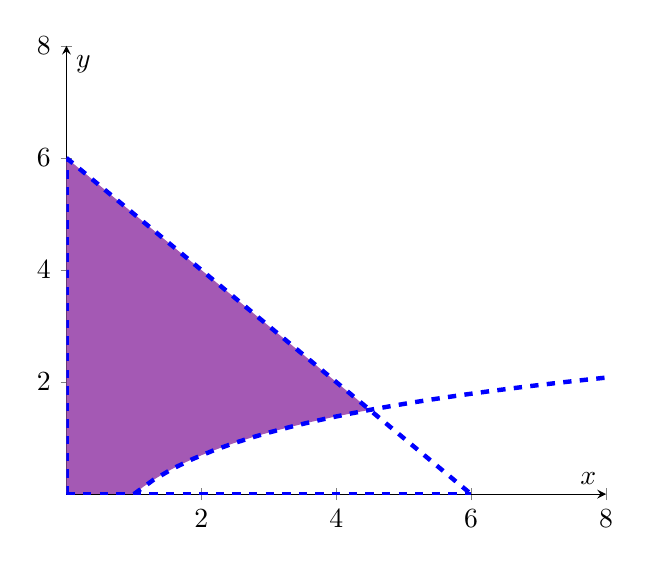
\begin{tikzpicture}[scale=1.0]
        \begin{axis}[
            axis x line=middle,
            axis y line=middle,
            ymin=0,ymax=8,ylabel=$y$,
            xmin=0,xmax=8,xlabel=$x$
        ]
            \begin{scope}
                \path[clip]
                    plot[domain=0:1] ({\x}, {0})
                    --plot[domain=1:4.49666] ({\x}, {ln(\x)})
                    --plot[domain=4.49666:0] ({\x}, {6-\x})
                    --plot[domain=0:6, variable=\y] ({0}, {\y})
                    --cycle;

                \fill [red!45!blue!65!] (0,0) rectangle (6,6);
            \end{scope}

            \plot[domain=0:6,blue,dashed,ultra thick] {6-\x};
            \plot[domain=1:8,blue,dashed,ultra thick] {ln(\x)};
            \plot[domain=0:6,blue,dashed,ultra thick] {0};
            \plot[domain=0:6,blue,dashed,ultra thick,variable=\y] ({0}, {\y});
        \end{axis}
    \end{tikzpicture}
\caption{Example feasible region (light purple) satisfying four constraints (dashed blue line)}
\label{fig:exmp-plant-feasible-region}
\end{figure}

\begin{exmp}
    Consider the problem of maximizing plant growth by manipulating quantities of two nutrients, $x_1$ and $x_2$. Let the plant height be $f(x_1, x_2) = 1 + x_1^2(x_2 - 1)^3e^{-x_1-x_2}$, with the constraints that $x_1 \geq 0$, $x_2 \geq 0$, $x_1 + x_2 \geq 6$, and $x_2 \geq \log x_1$. Then within the feasible region (depicted in Figure \ref{fig:exmp-plant-feasible-region}), $f$ is maximized by $(x_1, x_2) = (2, 4)$.
\end{exmp}

\begin{defn}
    For all $x \in \R^n$ and $\varepsilon > 0$, the \emph{$\varepsilon$-neighborhood} of $x$ is
    \[N_{\varepsilon}(x) = \left\{y \in \R^n \compbar \norm{x - y} < \varepsilon \right\}.\]
\end{defn}

\begin{exmp}
    In $\R^1$, $N_{3}(7)$ is $(4, 10)$.
\end{exmp}

\begin{defn}
    For any $S \subseteq \R^n$ and $x \in \R^n$, we say that $x$ is an \emph{interior point} of $S$ if there exists $N_{\varepsilon}(x) \subseteq S$. If every $N_{\varepsilon}(x)$ contains a point inside $S$ and a point not inside $S$, we say that $x$ is a \emph{boundary point} of $x$.
\end{defn}

\begin{defn}
    A set $S \subseteq \R^n$ is \emph{open} if every point in $S$ is an interior point of $S$, and \emph{closed} if $S$ contains every boundary point of $S$.
\end{defn}

\begin{exmp}
    In $\R^1$, any non-empty interval $[a, b]$ is closed, and non-empty $(a, b)$ is open.
\end{exmp}

\begin{exmp}
    Both $\emptyset$ and $\R^n \subseteq \R^n$ are both open and closed.
\end{exmp}

\begin{prop}
    Let $S \subseteq \R^n$. Then $S$ is open if and only if $\R^n - S$ is closed.
\end{prop}

\begin{proof}
    Assume that $S$ is open, and let $x$ be a boundary point of $\R^n - S$. Then for every $\varepsilon > 0$, by definition there exists $y, z \in N_{\varepsilon}(x)$ such that $y \in S$ and $z \in \R^n - S$. Therefore, $N_{\varepsilon}(x) \centernot\subseteq S$. It follows that $x \notin S$ by definition, and so $x \in \R^n - S$. Therefore, $\R^n - S$ contains every boundary point of itself, and so it is closed.

    Assume that $\R^n - S$ is closed, and let $x \in S$. Consider $N_{\varepsilon}(x)$. Since $\R^n - S$ contains all of its boundary points, $x$ cannot be a boundary point of $\R^n - S$, and so we know that there must be some $\varepsilon$ such that $N_{\varepsilon} \subseteq S$. Therefore, every $x \in S$ is an interior point of $S$, and so $S$ is closed by definition.
\end{proof}

\begin{exmp}
    We will examine a few cases in which minima and maxima may fail to first.

    \begin{itemize}
        \item Unbounded objective function, e.g. minimizing $\ln x$ such that $0 < x \leq 7$.
        \item Bounded objective function on open set, e.g. minimizing $\ln x$ such that $1 < x \leq 7$.
        \item Infeasible (feasible region is empty), e.g. minimizing $\ln x$ such that $1 < x$ and $x \leq 0.5$.
    \end{itemize}
\end{exmp}

\begin{exmp}
    When a solution exists, two distinct cases may occur.

    \begin{itemize}
        \item The solution is an interior point of the feasible region, e.g. minimizing $f(x) = 3 + (x - 2)^2$ such that $1 \leq x \leq 3$. The local minimum is $x^* = 2$, and $f'(x^*) = 0$.
        \item The solution is a boundary point of the feasible region, e.g. minimizing $f(x) = 3 + (x - 2)^2$ such that $x \leq 10$. Then $x^* = 10$, but $f'(x^*) \neq 0$.
    \end{itemize}
\end{exmp}

\begin{defn}
    Let $S \subseteq \R^n$ and $f: \R^n \to \R$. Consider $x^* \in S$. We say that $x^*$ is a \emph{global minimum} if for all $y \in S$, $f(x^*) \leq f(y)$, and a \emph{strict} global minimum if for all $y \in S - \{x^*\}$, $f(x^*) < f(y)$.
\end{defn}

\begin{defn}
    Let $S \subseteq \R^n$ and $f: \R^n \to \R$. Consider $x^* \in S$. We say that $x^*$ is a \emph{local minimum} if there exists an $\varepsilon$-neighborhood $N_{\varepsilon}(x^*)$ such that for all $y \in N_{\varepsilon}(x) \intersection S$, $f(x^*) \leq f(y)$, and a \emph{strict} local minimum if for all $y \in \left(N_{\varepsilon}(x) \intersection S\right) - \{x^*\}$, $f(x^*) < f(y)$.
\end{defn}

\begin{defn}
    Let $S \subseteq \R^n$ be a feasible region and $f: S \to \R$ an objective function. A \emph{stationary point} $x \in S$ is where $\nabla f(x) = \vec{0}.$
\end{defn}

\begin{rmk}
    Let $S \subseteq \R^n$, $x^*$ be an interior point of $S$, and $f: S \to \R$ be a sufficiently smooth continuous function. If $x^* \in S$ is a local minimum, then the \emph{gradient} of $f(x^*)$ is $\vec{0}$. However, $\nabla f(x^*) = \vec{0}$ does not imply that $x^*$ is a local minimum.
\end{rmk}

\subsection{Forms of Linear Programming Problems}

\begin{defn}
    A maximization or minimization linear programming problem in \emph{standard form} is a problem of the form:
    find $x \in \R^n$ that maximizes or minimizes $\transposeof{c}x$ such that $Ax = b$ and $x \geq \vec{0}$. The problem is said to be in \emph{canonical form} if the constraints are instead in the form $Ax \geq b$ (or $Ax \leq b$).
\end{defn}

\begin{exmp}
    Consider the problem of minimizing the cost per unit of chicken feed, while ensuring necessary nutrients are provided. Let $x_1, x_2, x_3, x_4$ denote the quantities of each of four ingredients, with cost per unit of $6.2$, $2.0$, $1.6$, and $3.2$ respectively. Let $n_1$, $n_2$, $n_3$ be the nutrients, with minimum required values of $6.2$, $11.9$, and $10.0$ respectively.

    \begin{minipage}{\linewidth}
        \begin{center}
        \captionof{table}{Nutrition values}
        \label{exmp-feed-nutrition-values}
        \begin{tabular}{c|cccc}
        & $x_1$ & $x_2$ & $x_3$ & $x_4$\\
        \hline
        $n_1$ & $1.2$ & $2.6$ & $0.0$ & $9.2$ \\ \hline
        $n_2$ & $3.9$ & $1.0$ & $0.8$ & $2.0$ \\ \hline
        $n_3$ & $6.0$ & $0.0$ & $4.0$ & $3.1$ \\
        \end{tabular}
        \end{center}
    \end{minipage}

    Let
    \[A = \begin{pmatrix}
        1.2 & 2.6 & 0.0 & 9.2 \\
        3.9 & 1.0 & 0.8 & 2.0 \\
        6.0 & 0.0 & 4.0 & 3.1
    \end{pmatrix},\; b = \begin{pmatrix}
        6.2 \\ 11.9 \\ 10.0
    \end{pmatrix},\; c = \begin{pmatrix}
        6.2 \\ 2.0 \\ 1.6 \\ 3.2
    \end{pmatrix},\; x = \begin{pmatrix}
        x_1 \\ x_2 \\ x_3 \\ x_4
    \end{pmatrix}\]
    then our problem is to minimize $\transposeof{c}x$ such that $Ax \geq b$ and $x \geq \vec{0}$. This form is the \emph{canonical form} of a linear programming problem.
\end{exmp}

\begin{rmk}
    We can easily convert problems expressed as a minimization problem into an equivalent maximization problem and vice versa, and between standard form and canonical form.
\end{rmk}

\begin{prop}
    Minimizing $\transposeof{c}x$ is equivalent to maximizing $-\transposeof{c}x$ (and so maximizing $\transposeof{c}x$ is equivalent to minimizing $-\transposeof{c}x$).
\end{prop}

\begin{proof}
    Let $P$ be a linear programming problem where we seek to minimize $\transposeof{c}x$, and let $S$ denote the feasible region of $P$. Now let $Q$ denote linear program where we seek to maximize $\transposeof{C}x$ that is otherwise identical to $P$. Let $x^{*}$ be a local minimum of $P$. By definition, there must exist some $\varepsilon$-neighborhood such that $\transposeof{c}x^{*} \leq \transposeof{c}y$ for all $y \in N_{\varepsilon}(x) \intersection S$. It follows that $-\transposeof{c}x^{*} \geq -\transposeof{c}y$ for all $y \in N_{\varepsilon}(x) \intersection S$, and so $x^{*}$ must be a local maximum of $Q$.
\end{proof}

\begin{prop}
    The constraint $Ax \geq b$ is equivalent to $-Ax \leq -b$, and $Ax \leq b$ is equivalent to $-Ax \geq -b$.
\end{prop}

\begin{prop}
    The constraint $Ax = b$ is equivalent to having both $Ax \geq b$ and $Ax \leq b$, and therefore is equivalent to $[A; -A] \geq [b; -b]$.
\end{prop}

\begin{prop}
    The constraint $Ax \geq b$ is equivalent to $Ax - z = b$, where $A \in M_{m \times n}(\R)$, $x \in \R^n$, and $z \in \R^m$ where $z \geq 0$. Here, $z$ is a vector of \emph{slack} variables.
\end{prop}

\begin{exmp}
    The constraints
    \begin{align*}
        a_{11}x_1 + a_{12}x_2 + a_{13}x_3 &\geq b_1 \\
        a_{21}x_1 + a_{22}x_2 + a_{23}x_3 &\geq b_2 \\
        a_{31}x_1 + a_{32}x_2 + a_{33}x_3 &\geq b_3 \\
        a_{41}x_1 + a_{42}x_2 + a_{43}x_3 &\geq b_4
    \end{align*}
    are equivalent to
    \begin{align*}
        a_{11}x_1 + a_{12}x_2 + a_{13}x_3 - x_4 &= b_1 \\
        a_{21}x_1 + a_{22}x_2 + a_{23}x_3 - x_5 &= b_2 \\
        a_{31}x_1 + a_{32}x_2 + a_{33}x_3 - x_6 &= b_3 \\
        a_{41}x_1 + a_{42}x_2 + a_{43}x_3 - x_7 &= b_4.
    \end{align*}
\end{exmp}

\begin{prop}
    We can incorporate the positivity constraints $x \geq 0$ into the general matrix constraints. The constraints $Ax \geq b$ and $x \geq 0$ are equivalent to \[\begin{bmatrix} A \\ I\end{bmatrix}x \geq \begin{bmatrix} b \\ 0 \end{bmatrix},\]
    and the constraints $Ax \leq b$ and $x \geq 0$ are equivalent to \[\begin{bmatrix} A \\ -I\end{bmatrix}x \leq \begin{bmatrix} b \\ 0 \end{bmatrix}.\]
\end{prop}

\begin{prop}
    We can transform an unconstrained problem into an equivalent problem with a positivity constraint.
\end{prop}

\begin{exmp}
    Consider the problem of minimizing $5x_1 + 6x_2$ such that $2x_1 - 3x_2 \geq 9$ and $x_1 + x_2 \geq -8$, with $x_1 \geq 0$ but $x_2$ unconstrained in sign. Define $x_2'$ and $x_2''$, and constrain $x_2', x_2'' \geq 0$. Let $x_2 = x_2' - x_2''$.
\end{exmp}

\begin{rmk}
    Constraints of the form $Ax = b$ are simply a system of equations, and therefore can be simplified using row operations by Theorem \ref{solutions-unchanged-by-row-ops}. Reduced row echelon form can help identified independent vs dependent variables.
\end{rmk}

\subsection{Polyhedrons}

\begin{defn}
    For non-zero $p \in \R^n$, the \emph{hyperplane} with normal vector $p$ is the orthogonal complement of $p$: \[\left\{x \in \R^n \compbar p \cdot x = 0 \right\},\]
    and the closed \emph{half-space} with normal vector $p$ is
    \[\left\{x \in \R^n \compbar p \cdot x \geq 0 \right\}.\]
    If we have $p \cdot x > 0$, we say it is an open half-space. We can replace $\geq$ and $>$ with $\leq$ and $<$ respectively.
\end{defn}

\begin{defn}
    A \emph{polyhedron} (or \emph{polyhedral set}) is the intersection of finitely many half spaces.
\end{defn}

\begin{defn}
    A polyhedron $P$ is \emph{bounded} if there exists $r \in \R$ such that $\norm{x} < r$ for all $x \in P$. A bounded polyhedron is known as a \emph{polytope}.
\end{defn}

\begin{prop}
    $P \subseteq \R^n$ is a polyhedron if and only if there exists $A \in M_{m \times n}(\R)$ and $b \in \R^m$ such that
    \[P = \left\{x \in \R^n \compbar Ax \geq b\right\}.\]
\end{prop}

\begin{defn}
    Let $X = \{x_1, \ldots, x_k\} \subset \R^n$. A \emph{convex combination} of $X$ is
    \[\lambda_1 x_1 + \lambda_2 x_2 + \cdots + \lambda_k x_k,\]
    where $\lambda_i \geq 0 \in \R$ and $\sum_{i=1}^{k}\lambda_i = 1$.
\end{defn}

\begin{defn}
    A set $S \subseteq \R^n$ is \emph{convex} if for any $x, y \in S$ and convex combination $z$ of $x$ and $y$, then $z \in S$.
\end{defn}

\begin{thm}
    Every polyhedron is convex.
\end{thm}

\begin{proof}
    Let $P = \left\{x \in \R^n, \compbar Ax \geq b\right\}$ be a polyhedron in $\R^n$. Let $x, y \in P$ and $z = \lambda x + (1 - \lambda) y$ be a convex combination of $x$ and $y$ for some $\lambda \in [0, 1]$.

    We know that $Ax \geq b$ and $Ay \geq b$, and want to show that $Az \geq b$. Since $z = \lambda x + (1 - \lambda)y$,
    \begin{align*}
        Az = A\left(\lambda x + (1 - \lambda)y\right) = \lambda Ax + (1 - \lambda)Ay \geq \lambda b + (1 - \lambda) b = b,
    \end{align*}
    and so $Az \geq b$.
\end{proof}

\begin{thm}
    A set $S \subseteq \R^n$ is convex if and only if every convex combination of every finite $X \subseteq S$ is in $S$.
\end{thm}

\begin{proof}
    We will prove this by showing that this is equivalent to the definition.
    
    $(\impliedby)$ If every convex combination of finite $X \subseteq S$ is in $S$, then every convex combination of $x, y \in S$ is in $X$.

    $(\implies)$ We will prove, via induction on $n = \abs{X}$, that if $z$ is a convex combination of $x, y \in S$ implies that $z \in S$, then every convex combination of $X \subseteq S$ is also in $S$.

    First, consider the base case of $n=1$, so $X = \{x\} \subseteq S$. The only convex combination of $X$ is simply $x$, and so every convex combination of $X$ is in $S$. Next, assume that if $z$ is a convex combination of $x, y \in S$ implies that $z \in S$, then every convex combination of $X \in S$ where $\abs{X} = n$ is also in $S$. For any $X' \subseteq S$ where $\abs{X'} = n+1$, there is some $X \subsetneq X'$ such that $\abs{X} = n$. Then every convex combination of $X$ is in $S$. Let \[\lambda_1x_1 + \cdots + \lambda_n x_n + \lambda_{n+1}x_{n+1}\] be a convex combination of $X$. Let $\Lambda = \lambda_1 + \cdots + \lambda_n$, and note that
    \[\alpha = \frac{\lambda_1}{\Lambda}x_1 + \cdots + \frac{\lambda_n}{\Lambda}x_n\] is a convex combination of $X$ and so must be in $S$ by by the induction hypothesis. Furthermore, note that
    \[\Lambda \alpha + \lambda_{n+1}x_{n+1}\] is our original convex combination of $X'$, but is also a convex combination of two points in $S$, and so is also in $S$ by assumption.
\end{proof}

\begin{defn}
    Let $S$ be a convex set, and consider $x \in S$. If $x$ being a convex combination of $y, z \in S$ implies that $x = y = z$, we say that $x$ is an \emph{extreme point}.
\end{defn}

\subsection{Basic Feasible Solutions}

\begin{defn}
    Let $c \in \R^n$, $A \in M_{m \times n}(\R)$, and $b \in \R^m$ be the linear program with feasibility region \[S = \left\{x \in \R^n \compbar Ax = b, x \geq \vec{0}\right\}.\] Let $A$ have rank $m$, or else eliminate redundant constraints until it does.

    Let $B$ be a subset of $m$ of the indices $\{1, \ldots, n\}$ such that the corresponding columns of $A$ form a basis for the column space of $A$ (which is $\R^m$ since $A$ has rank $m$). Let $A_B \in M_{m \times m}(\R)$ denote the invertible matrix of these columns.

    A \emph{basic feasible solution} is any $x \in S$ where $j \notin B$ implies $x_j = 0$.
\end{defn}

\begin{rmk}
    Without loss of generality, we can rearrange the columns of $A$ such that $A = [A_B | N]$, and then basic feasible solutions are precisely those $x \in S$ such that $x = \begin{bmatrix}
        x_B \\ x_N
    \end{bmatrix}$ where $x_N = \vec{0}$.
\end{rmk}

\begin{thm}
    Let $B \in M_{m \times m}(\R)$ have rank $m$, and $N \in M_{m \times (n-m)}(\R)$ where $m < n$, and then let $A = [B | N] \in M_{m \times n}(\R)$. Let $b \in \R^m$, so the feasible region is \[S = \left\{x \in \R^n \compbar Ax = b,\; x \geq \vec{0}\right\}.\]

    Then $x \in S$ is an extreme point of $S$ if and only if $x$ is a basic feasible solution of $S$.
\end{thm}

\begin{proof}\proofbreak
    ($\impliedby$) Suppose $x$ is a basic feasible solution of $S$, so $x = \begin{bmatrix}
        x_B \\ x_N
    \end{bmatrix}$ where $x_N = \vec{0}$. Let $x = \lambda x' + (1 - \lambda) x''$ be a non-trivial convex combination (so $0 < \lambda < 1$) of $x', x'' \in S$. We can represent $x'$ and $x''$ as $x' = \begin{bmatrix} x_B' \\ x_N' \end{bmatrix}$ and $x'' = \begin{bmatrix} x_B'' \\ x_N'' \end{bmatrix}$ respectively. Notice that we now have $x_N = \vec{0} = \lambda x_N' + (1 - \lambda)x_N''$. Since $x', x'' \in S$, we know $x_N', x_N'' \geq 0$ and so we necessarily have $x_N' = x_N'' = 0$. But then $x'$ and $x''$ are also basic feasible solutions. Since $A_{B}$ is invertible and $x, x', x'' \in S$, we know that $A_{B}x_B = A_{B}x_B'b = A_{B}x_B''$, and so $x = x' = x''$.

    ($\implies$) Suppose $x$ is not a basic feasible solution of $S$. Then $x = \begin{bmatrix}
        x_B \\ x_N
    \end{bmatrix}$ where $x_N$ is nonzero. We know that the columns of $A$ corresponding to the non-zero entries of $x$ must be linearly dependent, or else we can complete them to a basis for $\R^m$ and $x$ would be a basic feasible solution. Therefore, we know there exists non-zero $z$ such that $Az = \vec{0}$ and $z_i \neq 0$ implies $x_i \neq 0$. Note that for any $\alpha \in \R$, $A(x + \alpha z) = Ax + \alpha Az = b$, so any $x + \alpha z \geq \vec{0}$ is a feasible solution. Since $x_i$ is strictly greater than zero when $z_i \neq 0$, for sufficiently small $\varepsilon$ the points $x + \varepsilon z$ and $x - \varepsilon z$ must be feasible. Then $x = \frac{1}{2}\left(x + \varepsilon z\right) + \left(1 - \frac{1}{2}\right)\left(x - \varepsilon z\right)$, and so $x$ can be expressed as a non-trivial convex combination in $S$ and therefore is not extreme.
\end{proof}

\subsection{Simplex Method}

\begin{defn}
    Consider a linear program in standard form. Given a choice of basis $B$ such that $A = [B | N]$, the \emph{pre-tableau} is the matrix
    \begin{align*}
        \left[\begin{array}{c|c|c|c}
            1 & -\transposeof{c_B} & -\transposeof{c_N} & 0 \\
            \hline
            \vec{0} & B & N & b
        \end{array}\right].
    \end{align*}
    In other words, we have augment $A = [B|N]$ with the constraint values $b$, and then again with a new variable $z$ in the first column/row such that $z - \transposeof{c}x = 0$. Note that $z$ is therefore the value of the objective function.
\end{defn}

\begin{defn}
    Given a linear program in standard form, and basic feasible solution $\transposeof{x} = [\transposeof{x_B}, \vec{0}]$, the corresponding \emph{basic feasible simplex tableau} is the matrix
    \begin{align*}
        \left[\begin{array}{c|c|c|c}
            1 & 0 & \transposeof{c_B}B^{-1}N-\transposeof{c_N} & \transposeof{c_B}B^{-1}b \\
            \hline
            \vec{0} & I & B^{-1}N & B^{-1}b
        \end{array}\right].
    \end{align*}
\end{defn}

\begin{rmk}
    The basic feasible tableau is the reduced row echelon form of the pre-tableau. It can also be obtain by left-multiplying the pre-tableau by
    \begin{align*}
        \left[\begin{array}{c|c}
            1 & \transposeof{c_B}B^{-1} \\
            \hline
            \transposeof{\vec{0}} & B^{-1}
        \end{array}\right].
    \end{align*}
\end{rmk}

\begin{rmk}
    We can see that $z + (\transposeof{c_B}B^{-1}N-\transposeof{c_N})x_N = \transposeof{c_B}B^{-1}b$, so $z = \transposeof{c_B}B^{-1}b + (\transposeof{c_N} - \transposeof{c_B}B^{-1}N)x_N$. We often denote this as
    \[z = \transposeof{c_B}B^{-1}b + \transposeof{r_N}x_N,\]
    where
    \[\transposeof{r_N} = \transposeof{c_N} - \transposeof{c_B}B^{-1}N.\]
\end{rmk}

In the simplex, we start with a linear program $A, b, c$ in standard form. Assuming we already know a basis that leads to a basic feasible solution, we form the pre-tableau and either row-reduce or multiply through by the matrix from the above remark to obtain the basis feasible tableau.

To illustrate the linear program, we will consider
\begin{align*}
    A =
    \begin{bmatrix}
        2 & -1 & 3 & 7 & 1 & 2 & 8 \\
        5 & 2 & -8 & -1 & 2 & 0 & 1 \\
        4 & 6 & -2 & 4 & 1 & 3 & -5
    \end{bmatrix},\;\;
    b = \begin{bmatrix}
        2 \\ 4 \\ 3
    \end{bmatrix},\;\;
    \transposeof{c} = [6, -3, 2, 1, -1, 7, 1].
\end{align*}

We will use columns $1$, $3$, and $7$ as our basis columns, however we will leave the columns in their original order to make bookkeeping easier. Our pre-tableau is
\begin{align*}
    \left[\begin{array}{c|ccccccc|c}
        1 & -6 & 3 & -2 & -1 & 1 & -7 & -1 & 0 \\
        \hline
        0 & 2 & -1 & 3 & 7 & 1 & 2 & 8 & 2 \\
        0 & 5 & 2 & -8 & -1 & 2 & 0 & 1 & 4 \\
        0 & 4 & 6 & -2 & 4 & 1 & 3 & -5 & 3
    \end{array}\right].
\end{align*}

Row-reducing to the reduced row echelon form (while treating columns $1$, $3$, and $7$ as leading columns) brings us to our first basic feasible tableau:
\begin{align*}
    \left[\begin{array}{c|ccccccc|c}
        1 & 0 & 9.35 & 0 & 11.06 & 2.82 & -1.22 & 0 & 4.93 \\
        \hline
        0 & 1 & 1.03 & 0 & 1.62 & 0.31 & 0.82 & 0 & 0.81 \\
        0 & 0 & 0.33 & 1 & 1.14 & -0.05 & 0.50 & 0 & 0.01 \\
        0 & 0 & -0.51 & 0 & 0.04 & 0.07 & -0.14 & 1 & 0.04
    \end{array}\right].
\end{align*}

Now, we \emph{pivot} to a new (and improved!) basic feasible tableau by choosing a non-basis column to turn into a basis column. We make the greediest choice by choose the $4$th column ($5$th of the overall tableau) since it has the largest improvement to our objective function per unit change in the corresponding non-basis variable.

Letting $j = 4$, we choose the $k$th row (excluding the objective row on top) by \[\argmin_{k}\frac{b_k}{A_{kj}} \mathrm{ where } A_{kj} > 0.\] This gives us the $2$nd row, so we row-reduce again, replace the column whose leading term choose in the $2$nd row (which is column $3$) with column $4$. To do this, we treat column $4$ as if it was the second column while row-reducing. Our new basis columns are $1$, $4$, and $7$, giving us our second basic feasible tableau:
\begin{align*}
    \left[\begin{array}{c|ccccccc|c}
        1 & 0 & 6.14  & -9.67 & 0 & 3.29  & -6.01 & 0 & 4.81 \\
        \hline
        0 & 1 & 0.56  & -1.41 & 0 & 0.37  & 0.11  & 0 & 0.79 \\
        0 & 0 & 0.28  & 0.87  & 1 & -0.04 & 0.43  & 0 & 0.01 \\
        0 & 0 & -0.57 & -0.03 & 0 & 0.06  & -0.15 & 1 & 0.04
    \end{array}\right].
\end{align*}

Note that the objective function value has decreased from $4.93$ to $4.81$. We now continue pivoting in the manner, the objective function value decreasing from $4.81$, to $4.6$, to $-2.45$, to $-2.46$. When there are no positive entries in the objective function row (top row), there are no more improvements that can be made by changing our choice of basis and we have reached optimality.

\subsection{Two-Phase Method}

The Two-Phase Method is a technique for coming up with the initial basic feasible solution need to start off the Simplex Method. In Phase I, we solve a different linear program to find the initial basic feasible solution, and then in Phase II we use that basic feasible solution to apply the simplex method to the original linear program. We take a problem in standard form with constraints $Ax = b$, $x \geq 0$ where $A \in M_{m \times n}(\R)$. We then introduce \emph{artificial variables} $x_{n+1}, x_{n+2}, \ldots, x_{n+m}$ for each constraint (row) in $A$. Let $x'$ denote the vector obtained by appending the artificial variables to $x$.

For Phase I, we solve a different problem using the Simplex Method: minimizing $x_{n+1} + x_{n+2} + \cdots + x_{n+m}$ such that $[A|I]x' = b$, $x' \geq 0$. Notice that any feasible solution to this new problem is a feasible solution to the original linear program if the objective function value is zero. Therefore, the $x$ part of an optimal solution $x'$ to the new problem is a feasible solution to the original if $x'$ has objective function value zero. If the optimal solution $x'$ has a positive objective function value, then no feasible solution exists for the original linear program.

Note that
\begin{align*}
    x' = \begin{bmatrix}
        x \\
        x_{n+1} \\
        \vdots \\
        v_{n+m}
    \end{bmatrix} = \begin{bmatrix}
        0 \\
        b_1 \\
        \vdots \\
        b_m
    \end{bmatrix}
\end{align*}
is always a basic feasible solution to the Phase I problem. Therefore, we can immediately apply the Simplex method to determine the feasibility of the original linear program, and find a feasible solution if one exists. Additionally, since the number of columns in a basis for either linear program is the same (always just $m$), the feasible solution given to us by Phase I must in fact be a basic feasible solution for Phase II.

\subsection{Big-M Method}

In the Big-M method, we essentially combine the two phases of the Two-Phase method by using the objective function
\begin{align*}
    \transposeof{c}x + M(x_{n+1} + x_{n+2} + \cdots + x_{n+m}),
\end{align*}
where $M$ is a very large value. This penalizes the artificial variables and causes them to be zero in any optimal solution. Setting the artificial variables to $b$ gives us an initial basic feasible solution. If a basic feasible solution exists where the artificial variables are zero, the first $m$ pivots will replace each artificial variable with non-artificial variables, and so the final optimal solution will be a solution to the original linear program.

\subsection{Duality}

\begin{defn}{Canonical or symmetric duality}\proofbreak
    Consider a linear program of the form minimize $\transposeof{c}x$ such that $Ax \geq b$ and $x \geq \vec{0}$. The \emph{dual} problem is maximizing $\transposeof{b}y$ such that $\transposeof{A}y \leq c$ and $y \geq \vec{0}$. The original linear program is referred to as the \emph{primal} probem in relation to its dual.
\end{defn}

\begin{exmp}
    Consider minimizing $1x_1 + 2x_2$ such that
    \begin{align*}
        3x_1 + 4x_2 &\geq 9, \\
        5x_1 + 6x_2 &\geq 10, \\
        7x_1 + 8x_2 &\geq 11, \\
        x_1, x_2 &\geq 0.
    \end{align*}

    The dual problem is maximizing $9y_1 + 10y_2 + 11y_3$ such that
    \begin{align*}
        3y_1 + 5y_2 + 7y_3  &\leq 1, \\
        4y_1 + 6y_2 + 8y_3  &\leq 2, \\
        y_1, y_2, y_3 &\geq 0.
    \end{align*}
\end{exmp}

\begin{defn}{Standard duality}\proofbreak
    Consider a linear program of the form minimization of $\transposeof{c}x$ such that $Ax = b$ and $x \geq \vec{0}$. The \emph{dual} problem is maximizing $\transposeof{b}y$ such that $\transposeof{A}y \leq c$, \emph{without} a non-negativity constraint on $y$. The original linear program is again referred to as the \emph{primal} probem in relation to its dual.
\end{defn}

\begin{rmk}
    We can derive the canonical form of duality from the standard form, and vice versa. Imagine we know that the dual of minimizing $\transposeof{c}x$ such that $Ax = b$ and $x \geq \vec{0}$ was to maximize $\transposeof{b}y$ such that $\transposeof{A}y \leq c$. If we were now given a linear program in canonical form and wanted to find its dual, we could first convert it into standard form by the introduction of slack variables, obtaining minimize $\transposeof{c}x$ such that $[A|-I]\begin{bmatrix}x \\ z\end{bmatrix} = b$ such that $\begin{bmatrix}x \\ z\end{bmatrix} \geq 0$. The standard dual of this is to maximize $\transposeof{b}y$ such that $\transposeof{[A|-I]}y \leq \begin{bmatrix}c \\ \vec{0}\end{bmatrix}$, which is equivalent to maximizing $\transposeof{b}y$ such that $\transposeof{A}y \leq c$ and $y \geq \vec{0}$ (from $-y \leq \vec{0}$).
\end{rmk}

\begin{prop}
    The canonical and standard duals of equivalent linear programs are equivalent.
\end{prop}

\begin{proof}
    See figure \ref{fig:duality-equivalence}.
\end{proof}

\begin{figure}[ht]
    \centering
    \begin{tikzpicture}[{baseline=(current bounding box.north)}]
        \node[align=center] at (-3,2.5) {$
            \begin{aligned}
                \mathrm{min.}\;\transposeof{c}&x \\
                \mathrm{s.t.}\;A&x \geq b, \\
                        &x \geq \vec{0}.
            \end{aligned}
        $};
        \node[align=center] at (3,2.5) {$
            \begin{aligned}
                \mathrm{max.}\;\transposeof{b}&y \\
                \mathrm{s.t.}\;\transposeof{A}&y \leq c, \\
                        &y \geq \vec{0}.
            \end{aligned}
        $};
        \node[align=center] at (-3,-3) {$
            \begin{aligned}
                \mathrm{min.}\;\transposeof{\begin{bmatrix}c \\ \vec{0}\end{bmatrix}}&\begin{bmatrix}x \\ z\end{bmatrix} \\
                \mathrm{s.t.}\;\left[A|-I\right]&\begin{bmatrix}x \\ z\end{bmatrix} = b, \\
                        &x, z \geq \vec{0}.
            \end{aligned}
        $};
        \node[align=center] at (3,-3) {$
            \begin{aligned}
                \mathrm{max.}\;&\transposeof{b}y \\
                \mathrm{s.t.}\;&\begin{bmatrix}\transposeof{A} \\ -I\end{bmatrix}y \leq \begin{bmatrix}c \\ \vec{0}\end{bmatrix}.
            \end{aligned}
        $};

        \draw[ultra thick, blue, ->] (-1, 3) -- (1, 3);
        \draw[ultra thick, red, ->] (-1, -3) -- (1, -3);
        \draw[ultra thick, black, <->] (3, -1) -- (3, 1);
        \draw[ultra thick, black, <->] (-3, 1) -- (-3, -1);

    \end{tikzpicture}
\caption{Equivalence of dualities}
\label{fig:duality-equivalence}
\end{figure}

\newpage

\begin{prop}
    Given a primal linear program, the dual of the dual is the primal.
\end{prop} 

\begin{proof}
    Consider a linear program in canonical form.  By definition, the dual is maximizing $\transposeof{b}y$ such that $\transposeof{A}y \leq c$ and $y \geq 0$. This program is equivalent to minimizing $-\transposeof{b}y$ such that $-\transposeof{A}y \geq -c$ and $y \geq 0$. The dual of this equivalent form of the dual is to maximizing $-\transposeof{c}x$ such that $\transposeof{\left(-\transposeof{A}\right)}x \leq -b$ and $x \geq 0$. Finally, this program is equivalent to minimizing $\transposeof{c}x$ such that $Ax \geq b$ and $x \geq 0$, which is the primal linear program.
\end{proof}

\begin{thm}{Weak Duality}\label{weak-duality}\proofbreak
    Consider a linear program and its dual, and $x, y$ feasible solutions to the primal and dual programs respectively. Then the objective function value at $y$ in the dual is less than or equal to the objective function value at $x$ in the primal.
\end{thm}

\begin{proof}
    When the primal is in standard form, we have $Ax = b$, $x \geq \vec{0}$ and $\transposeof{A}y \leq c$. It follows that $\transposeof{b}y = \transposeof{(Ax)}y = \transposeof{x}\transposeof{A}y$. Since we have $x \geq \vec{0}$, we know that $\transposeof{x}\transposeof{A}y \leq \transposeof{x}c$, and so $\transposeof{b}y \leq \transposeof{c}x$.

    When the primal is in canonical form, we have $Ax \geq b$, $x \geq \vec{0}$, $\transposeof{A}y \leq c$, and $y \geq 0$. Since $y \geq \vec{0}$, $Ax \geq b$ implies that $\transposeof{b}y \leq \transposeof{(Ax)}y$, and so $\transposeof{b}y \leq \transposeof{x}\transposeof{A}y$. Furthermore, since $\transposeof{A}y \leq c$ and $x \geq \vec{0}$, $\transposeof{x}\transposeof{A}y \leq \transposeof{x}c = \transposeof{c}x$. Combining these, we arrive at $\transposeof{b}y \leq \transposeof{c}y$.
\end{proof}

\begin{cor}
    The optimal objective value function in the dual is less than or equal to the optimal objective function value in the primal.
\end{cor}

\begin{cor}{Supervisor principle}\label{supervisor-principle}\proofbreak
    If $\transposeof{b}y = \transposeof{c}x$, then $x$ and $y$ are optimal in their respective linear programs.
\end{cor}

\begin{thm}{Strong Duality}\label{strong-duality}\proofbreak
    Suppose a linear program has a feasible solution and its objective function is bounded from below. Then the linear program and its dual have optimal solutions $x$ and $y$ respectively, and the objective function value of $x$ and $y$ are equal.
\end{thm}

\begin{proof}
    Consider the primal in standard form. We can apply the Simplex method or similar to obtain an optimal basic feasible solution $x^*$. Without loss of generality, we can assume that the final basis consists of the first $m$ columns of $A$.

    By the terminating condition of the Simplex method, we know that
    \begin{align*}
        \transposeof{r_N} = \transposeof{c_N} - \transposeof{c_B}B^{-1}N \geq \vec{0}.
    \end{align*}
    Let
    \begin{align*}
        \transposeof{y^*} = \transposeof{c_B}B^{-1}.
    \end{align*}

    Since $\transposeof{r_N} \geq \vec{0}$, we know that
    \begin{align*}
        \transposeof{c_B}B^{-1}N \leq \transposeof{c_N},
    \end{align*}
    and so it follows that
    \begin{align*}
        \transposeof{y^*}A = \transposeof{c_B}B^{-1}[B|N] = [\transposeof{c_B}|\transposeof{c_B}B^{-1}N] \leq [\transposeof{c_B}|\transposeof{c_N}] = \transposeof{c},
    \end{align*}
    so $y^*$ is a feasible solution to the dual. Now we can show that the objective function values are equal:
    \begin{align*}
        \transposeof{y^*}b = \transposeof{c_B}B^{-1}b = \transposeof{\begin{bmatrix}c_B \\ \vec{0}\end{bmatrix}}\begin{bmatrix}x_B \\ \vec{0}\end{bmatrix} = \transposeof{c}x^*.
    \end{align*}

    Therefore, $y^*$ is an optimal solution to the dual linear program by the supervisor principle \ref{supervisor-principle}.
\end{proof}

\subsection{Sensitivity Analysis}

\begin{defn}
    A basic feasible solution $b$ to a linear program with basis $B$ is \emph{non-degenerate} when $B^{-1}b > \vec{0}$.
\end{defn}

Consider solving a linear program $A, b, c$ in standard form by the Simplex method. What happens if we replace $b$ with $b' = b + \Delta b$ for some arbitrary $\Delta b$? If we replaced $B^{-1}b$ with $B^{-1}(b + \Delta b)$ and $\transposeof{c_B}B^{-1}b$ with $\transposeof{c_B}B^{-1}(b + \Delta b)$ in just the final basic feasible simplex tableau, what happens?

If $B^{-1}(b + \Delta b) \geq \vec{0}$, then we still have a basic feasible solution! Furthermore, since the objective row would still be non-positive, our solution would also be an \emph{optimal} basic feasible solution. This would very likely only occur when $\Delta b$ is fairly small.

If the linear program is non-degenerate, there always exists such $\Delta b$ small enough.

In the corresponding dual linear program, we know that
\begin{align*}
    \transposeof{y^*} = \transposeof{c_B}B^{-1}.
\end{align*}
We also have $\transposeof{c}x^* = \transposeof{y^*}b$, and so when we replace $b$ with $b'$ we get
$\transposeof{c}{x'}^{*} = \transposeof{y^*}(b + \Delta b) = \transposeof{y^*}b + \transposeof{y^*}\Delta b$. Therefore,
\begin{align*}
    \frac{\transposeof{c}{x'}^{*}}{\partial b_i} = y_i^*.
\end{align*}

\begin{defn}
    Vectors $x, y \in \R^n$ are \emph{complementary} if $x_i \neq 0 \implies y_i = 0$ and $y_i \neq 0 \implies x_i = 0$.
\end{defn}

\begin{prop}\label{complementary-orthogonal}
    If $x \geq 0$ and $y \geq 0$, then $x$ and $y$ are complementary if and only if $\transposeof{x}y = 0$.
\end{prop}

\begin{proof}
    If $x$ and $y$ are complementary, then $x_iy_i = 0$, and so $\transposeof{x}y = 0$.

    Since $x \geq 0$ and $y \geq 0$, we know $x_iy_i \geq 0$. If $\transposeof{x}y = 0$, then we must have $x_iy_i = 0$. Therefore at least one of $x_i$ and $y_i$ is zero and so $x$ and $y$ are complementary.
\end{proof}

\begin{thm}{Complementary slackness}\label{complementary-slackness}\proofbreak
    Consider a linear program $A, b, c$ in standard form. Let $x \in \R^n$ be a feasible solution. Let $y \in \R^m$ be a feasible solution in the dual. Then $x$ and $y$ are optimal solutions if and only if $c - \transposeof{A}y$ is complentary to $x$.
\end{thm}

\begin{proof}
    Recall that
    \begin{align*}
        \transposeof{b}y = \transposeof{(Ax)}y = \transposeof{x}\transposeof{A}y \leq \transposeof{x}c = \transposeof{c}x.
    \end{align*}
    By the supervisor principle \ref{supervisor-principle}, $x$ and $y$ are optimal if and only if $\transposeof{b}y = \transposeof{c}x$, which is equivalent to $\transposeof{x}\transposeof{A}y = \transposeof{x}c$. Therefore,
    \begin{align*}
        \transposeof{x}\left(c - \transposeof{A}y\right) = \vec{0}.
    \end{align*}

    Since $y$ is feasible in the dual, by definition $\transposeof{A}y \leq c$, and so $c - \transposeof{A}y \geq \vec{0}$. Furthermore, $x \geq 0$ and so by Proposition \ref{complementary-orthogonal} it follows that this occurs precisely when $x$ and $c - \transposeof{A}y$ are complementary.
\end{proof}

\subsection{Dual Simplex Method}

In the dual simplex method, we have a linear program in standard form. Unlike when we start the simplex method, rather than knowing a starting feasible solution and working towards optimality, we know a starting solution that is essentially optimal and works towards feasibility. We actually start with a vector $y$ that is feasible in the dual linear program, and work towards making the corresponding primal vector $x$ feasible in the primal. Due to the setup of the dual simplex method, both $y$ and $x$ will have the same objective function value, and so once $x$ is feasible we have an optimal solution by the supervisor principle \ref{supervisor-principle}.

\begin{defn}{Basic tableau}\proofbreak
    A basic tableau is a tableau formed from a basic, but not necessarily feasible, solution.
\end{defn}

Given a linear program in standard form and corresponding basic tableau, we have $\transposeof{y} = \transposeof{c_B}B^{-1}$ and $x = B^{-1}b$. Recall that $y$ is an optimal solution to the dual problem when:
\begin{itemize}
    \item $Ax = b$,
    \item $x \geq 0$,
    \item $\transposeof{A}y \leq c$,
    \item $\transposeof{c}x = \transposeof{b}y$.
\end{itemize}

The first condition, that $Ax = b$ is necessarily satisfied by any basic tableau. The fourth, that $\transposeof{c}x = \transposeof{b}y$, is also satisfied since $\transposeof{c_B}B^{-1}b = \transposeof{y}b = \transposeof{b}y$ and $\transposeof{c_B}B^{-1}b = \transposeof{c}x$. The third condition, that $\transposeof{A}y \leq c$, is satisfied when $r \geq 0$. Since the top row of the tableau is $-r$, to have dual feasibility at the start of the dual simplex method we require that $-r \leq 0$ --- that is, that the top row of the basic tableau is non-positive other than the constant $1$. Therefore, we need to come up with a ``dual pivot'' that preserves these properties while working towards achieving the second condition.

To dual pivot, we choose the row $j$ with the most-negative value in $B^{-1}b$, and pick a column to row-reduce on. Since we need to maintain a non-positive top row $-r$, we want to pick the column $k$ by \[\argmin_{k}\frac{r_k}{A_{jk}} \mathrm{ where } A_{jk} < 0.\]

\section{Non-Linear Programming}

\begin{defn}
    Let $S \subseteq \R^n$ be a non-empty convex set, and let $f: S \to \R$. We say that $f$ is \emph{convex} when
    \begin{align*}
        f\left(\lambda x + (1 - \lambda)y\right) \leq \lambda f(x) + (1 - \lambda)f(y)
    \end{align*}
    for all $x, y \in S$ and $\lambda \in [0, 1]$.

    Similarly, we say that $f$ is \emph{strictly convex} when
    \begin{align*}
        f\left(\lambda x + (1 - \lambda)y\right) < \lambda f(x) + (1 - \lambda)f(y)
    \end{align*}
    for all $x, y \in S$ and $\lambda \in (0, 1)$.

    We analogously define \emph{concave} and \emph{strictly concave} functions using $\geq$ and $>$ respectively.
\end{defn}

\begin{rmk}
    Note that we use an open interval for $\lambda$ in the strict case, and a closed interval otherwise. This is because at $\lambda = 0$ or $\lambda = 1$ we will always have equality.
\end{rmk}

\begin{defn}
    Let $S \subseteq \R^n$, and consider $f: S \to \R$. The \emph{epigraph} of $f$ 
    \begin{align*}
        \left\{\begin{bmatrix}
            x \\ y
        \end{bmatrix} \compbar x \in S, y \in R, y \geq f(x)\right\} \subseteq \R^{n+1}
    \end{align*}
    and is denoted by $\epigraph(f)$. That is, the epigraph is all points above the graph of the function.
\end{defn}

\begin{prop}\label{epigraph-convexity}
    Let $S \subseteq \R^n$, and consider $f: S \to \R$. Then $f$ is a convex function if and only if $\epigraph(f)$ is a convex set.
\end{prop}

\begin{proof}\proofbreak
    ($\implies$) Assume that $f$ is convex. Then for any $\transposeof{[x_1, y_1]}, \transposeof{[x_2, y_2]} \in \epigraph(f)$ and $\lambda \in [0, 1]$, we know that
    \begin{align*}
        f(\lambda x_1 + (1 - \lambda)x_2) \leq \lambda f(x_1) + (1 - \lambda)f(x_2) \leq \lambda y_1 + (1 - \lambda)y_2.
    \end{align*}
    Therefore,
    \begin{align*}
        \lambda \begin{bmatrix}
            x_1 \\ y_1
        \end{bmatrix} + (1-\lambda)\begin{bmatrix}
            x_2 \\ y_2
        \end{bmatrix} = \begin{bmatrix}
            \lambda x_1 + (1 - \lambda)x_2 \\
            \lambda y_1 + (1 - \lambda)y_2
        \end{bmatrix} \in \epigraph(f),
    \end{align*}
    and so $\epigraph(f)$ is a convex set.

    ($\impliedby$) Assume that $\epigraph(f)$ is a convex set. Since we trivially have $f(x) \leq f(x)$ for all $x \in S$, we know that for any $x_1, x_2 \in S$ we have
    \begin{align*}
        \transposeof{[x_1, f(x_1)]}, \transposeof{[x_2, f(x_2)]} \in \epigraph(f).
    \end{align*}
    Since $\epigraph(f)$ is convex, for all $\lambda \in [0, 1]$ we also know that
    \begin{align*}
        \lambda \begin{bmatrix}
            x_1 \\ f(x_1)
        \end{bmatrix} + (1-\lambda)\begin{bmatrix}
            x_2 \\ f(x_2)
        \end{bmatrix} = \begin{bmatrix}
            \lambda x_1 + (1 - \lambda)x_2 \\
            \lambda f(x_1) + (1 - \lambda)f(x_2)
        \end{bmatrix} \in \epigraph(f).
    \end{align*}
    Therefore,
    \begin{align*}
        f(\lambda x_1 + (1 - \lambda)x_2) \leq \lambda f(x_1) + (1-\lambda)f(x_2)
    \end{align*}
    by the definition of $\epigraph(f)$, and so $f$ is a convex function.
\end{proof}

\begin{thm}{Support Theorem}\label{support-theorem}\proofbreak
    Let $S \subseteq \R^n$ be a convex set, and let $\bar{x}$ be a boundary point of $S$. There exists a hyperplane containing $\bar{x}$ such that $S$ is contained in an associated closed half-space.
\end{thm}

\begin{thm}\label{convex-function-tangent-hyperplane}
    Let $S \subseteq \R^n$ be an open convex set, and let $f: S \to \R$ be continuously differentiable. Then $f$ is a convex function if and only if
    \begin{align*}
        f(x) \geq f(\bar{x}) + \transposeof{\nabla f(\bar{x})}(x - \bar{x})
    \end{align*}
    for all $x, \bar{x} \in S$. 
\end{thm}

\begin{thm}
    Let $S \subseteq \R^n$ be an open convex set, and let $f: S \to \R$ be continuously differentiable. Then $f$ is strictly convex if and only if 
    \begin{align*}
        f(x) > f(\bar{x}) + \transposeof{\nabla f(\bar{x})}(x - \bar{x})
    \end{align*}
    for all $x, \bar{x} \in S$ where $x \neq \bar{x}$. 
\end{thm}

\begin{cor}
    Let $S \subseteq \R^n$ be an open convex set, and let $f: S \to \R$ be \emph{twice} continuously differentiable. Then $f$ is convex if and only if $\nabla^2f(\bar{x})$ is positive semi-definite for all $\bar{x} \in S$.
\end{cor}

\begin{proof}\proofbreak
    Assume $\nabla^2f(\bar{x})$ is positive semi-definite for all $\bar{x} \in S$. By Taylor's theorem, for all $x \in S$ we have
    \begin{align*}
        f(x) = f(\bar{x}) + \transposeof{\nabla f(\bar{x})}(x - \bar{x}) + \frac{1}{2}\transposeof{(x - \bar{x})}\nabla^2f(z)(x - \bar{x})
    \end{align*}
    for some $z \in S$. Since $\nabla^2f(\bar{x})$ is positive semi-definite, we know that $\frac{1}{2}\transposeof{(x - \bar{x})}\nabla^2f(z)(x - \bar{x}) \geq 0$, and so we have
    \begin{align*}
        f(x) \geq f(\bar{x}) + \transposeof{\nabla f(\bar{x})}(x - \bar{x}).
    \end{align*}

    Now assume $\nabla^2f(\bar{x})$ is \emph{not} positive semi-definite for all $\bar{x} \in S$. Then there exists $d \in \R^n$ such that $\transposeof{d}\nabla^2f(\bar{x})d < 0$. By continuity of $\nabla^2f(\bar{x})$, there is a neighborhood around $\bar{x}$ such that $\transposeof{d}\nabla^2f(z)d < 0$ for all $z$ in that neighborhood. By Taylor's theorem, for all $x \in S$ we have
    \begin{align*}
        f(x) = f(\bar{x}) + \transposeof{\nabla f(\bar{x})}(x - \bar{x}) + \frac{1}{2}\transposeof{(x - \bar{x})}\nabla^2f(z)(x - \bar{x})
    \end{align*}
    for some $z \in S$. Choose $x = \bar{x} + \alpha d$ for $\alpha > 0$ small enough that $x$ is in that neighborhood, and since $z$ falls between $x$ and $\bar{x}$, $z$ is also in that neighborhood. Then $\frac{1}{2}\transposeof{(x - \bar{x})}\nabla^2f(z)(x - \bar{x}) < 0$, and so we have
    \begin{align*}
        f(x) < f(\bar{x}) + \transposeof{\nabla f(\bar{x})}(x - \bar{x}).
    \end{align*}
\end{proof}

\begin{prop}
    Let $S \in \R^n$ be an open convex set, and let $f: S \to \R$ be a continuously differentiable convex function. Then for any $\bar{x} \in S$, the following are equivalent:
    \begin{itemize}
        \item $\bar{x}$ is a global minimum,
        \item $\bar{x}$ is a local minimum,
        \item $\bar{x}$ is stationary point.
    \end{itemize}
\end{prop}

\begin{proof}
    If $\bar{x}$ is a global minimum, then $\bar{x}$ is a local minimum. If $\bar{x}$ is a local minimum, then $\bar{x}$ is a stationary point. Therefore, we only need to show that stationary points are global minimums, and the result will follow.

    By convexity of $f$, for all $x \in S$ we know that $f(x) \geq f(\bar{x}) + \transposeof{\nabla f(\bar{x})}(x - \bar{x})$ by Theorem \ref{convex-function-tangent-hyperplane}. If $\bar{x}$ is a stationary point, then $\nabla f(\bar{x})$ by definition, and so $f(x) \geq f(\bar{x})$. Then $\bar{x}$ is a global minimum by definition.
\end{proof}

\begin{defn}{Newton's Method}\label{newtons-method}\proofbreak
    Let $f: \R^n \to \R$ be twice continuously differentiable, and pick some $x^{(0)} \in \R^n$. For $i = 1, 2, \ldots, $ while $f(x^{(i)}) \neq 0$ (or until some other terminating condition), let
    \begin{align*}
        x^{(i+1)} = x^{(i)} - \left(\nabla^2f(x^{(i)})\right)^{-1}\nabla f(x^{(i)}).
    \end{align*}
\end{defn}

\begin{rmk}
    Assume that $\nabla^2f$ is constant, and that all derivatives of $f$ of order higher than two are zero. Then a local minimum occurs when $\nabla^2f(x) = 0$, and so we want $\nabla f(x^{(i+1)}) = 0$. Since the higher derivatives are zero,
    \begin{align*}
        \nabla f(x^{(i+1)}) = \nabla f(x^{(i)}) + \nabla^2f(x^{(i)})(x^{(i+1)} - x^{(i)}).
    \end{align*}
    Therefore, if we want the gradient to be zero, we have
    \begin{align*}
        0 &= \nabla f(x^{(i)}) + \nabla^2f(x^{(i)})(x^{(i+1)} - x^{(i)}) \\
        x^{(i+1)} - x^{(i)} &= -\left(\nabla^2f(x^{(i)})\right)^{-1}\nabla f(x^{(i)}) \\
        x^{(i+1)} &= x^{(i)} - \left(\nabla^2f(x^{(i)})\right)^{-1}\nabla f(x^{(i)}).
    \end{align*}
    While our assumptions will almost certainly be invalid, making these ``Newton steps'' will often produce rapid progress towards a local minimum. For non-pathological functions, the closer to the local minimum the better our linear approximation of $\nabla f$ will be.
\end{rmk}

\begin{defn}{Steepest Descent}\label{steepest-method}\proofbreak
    Let $f: \R^n \to \R$ be continuously differentiable, and pick some $x^{(0)} \in \R^n$. 
    For $i = 1, 2, \ldots, $ while $f(x^{(i)}) \neq 0$ (or until some other terminating condition), define
    \begin{align*}
        g(\alpha) = f(x^{(i)} - \alpha\nabla f(x^{(i)})),
    \end{align*}
    and then let
    \begin{align*}
        \alpha^* &= \argmin_{\alpha}g(\alpha) \\
        x^{(i+1)} &= x^{(i)} - \alpha^{*}\nabla f(x^{(i)}).
    \end{align*}
\end{defn}

\subsection{Karush-Kuhn-Tucker Conditions}

\begin{thm}{Farkas' Theorem}\label{farkas}\proofbreak
    Let $A \in M_{m \times n}(\R)$, $b \in \R^m$. Then exactly one of the following is true:
    \begin{itemize}
        \item there exists $x \in \R^n$ such that $Ax = b$ and $x \geq \vec{0}$,
        \item there exists $y \in \R^m$ such that $\transposeof{b}y > 0$ and $\transposeof{A}y \leq \vec{0}$.
    \end{itemize}
\end{thm}

\begin{proof}
    Consider the linear program of minimizing $\transposeof{\vec{0}}x$ such that $Ax = b$ and $x \geq {0}$. The dual program is maximizing $\transposeof{b}y$ such that $\transposeof{A}y \leq \vec{0}$.

    In the first case, the primal program is feasible and the objective function value at $x$ is necessarily zero. Then by Weak Duality \ref{weak-duality}, we know that the dual program has no feasible solution with objective function value greater than zero, and so the second case cannot be true.

    If the second case is false, then the dual program has no feasible solutions with positive objective function value. We know however that the $y = \vec{0}$ is a feasible solution to the dual with objective function value of zero, and is therefore the optimal solution. By Strong Duality \ref{strong-duality}, the primal program must have a feasible solution $x$, and so the first case is true.
\end{proof}

\begin{thm}{Gordon's Theorem}\label{gordons}\proofbreak
    Let $A = M_{m \times n}(\R)$. Then exactly one of the following is true:
    \begin{itemize}
        \item there exists $x \in \R^n$ such that $Ax = \vec{0}$, $x \geq \vec{0}$, $x \neq \vec{0}$.
        \item there exists $y \in \R^m$ such that $\transposeof{A}y < \vec{0}$.
    \end{itemize}
\end{thm}

\begin{proof}
    Assume the second case is true, so there exists $y \in \R^m$ such that $\transposeof{A}y < \vec{0}$. Equivalently, there exists $\varepsilon > 0$ such that $\transposeof{A}y + \varepsilon\vec{1} \leq \vec{0}$ --- that is, there exists
    \begin{align*}
        \begin{bmatrix}
            y \\ \varepsilon
        \end{bmatrix} \in \R^{m+1}
    \end{align*}
    such that
    \begin{align*}
        \transposeof{\begin{bmatrix}
            \vec{0} \\ 1
        \end{bmatrix}}
        \begin{bmatrix}
            y \\ \varepsilon
        \end{bmatrix} > 0,\;\;\;\begin{bmatrix}
            \transposeof{A} | \vec{1}
        \end{bmatrix}\begin{bmatrix}
            y \\ \varepsilon
        \end{bmatrix} \leq \vec{0}.
    \end{align*}
    By Farkas \ref{farkas}, this is true if and only if there is no $x \geq \vec{0}$ such that
    \begin{align*}
        \begin{bmatrix}
            A \\ \transposeof{\vec{1}}
        \end{bmatrix}x = \begin{bmatrix}
            \vec{0} \\ 1
        \end{bmatrix}.
    \end{align*}
    This is in turn equivalent to
    \begin{align*}
        Ax = \vec{0},\;\;\;x \geq \vec{0}\;\;\;\transposeof{\vec{1}}x = 1.
    \end{align*}
    Note that this is equivalent to the first case from this theorem: the existence of such $x \neq 0$ implies the existence of
    \begin{align*}
        x' = \frac{1}{\transposeof{\vec{1}}x}x,
    \end{align*}
    and we would have $Ax' = \frac{1}{\transposeof{\vec{1}}x}\vec{0} = \vec{0}$, $x' \geq \vec{0}$, $\transposeof{\vec{1}}x' = 1$.

    Therefore, the second case is equivalent to the negation of the first, and so exactly one of them is true for any $A$.
\end{proof}

\begin{rmk}
    From here until the Karush-Kuhn-Tucker Conditions, let $P$ be the problem of minimizing $f(x)$ such that $g_i(x) \leq 0$ for $i = 1, \ldots, m$ where $f: \R^n \to \R$ and $g_i: \R^n \to \R$ are continuously differentiable.
\end{rmk}

\begin{defn}
    For all feasible $x \in \R^n$, the \emph{active constraints} at $x$ are
    \begin{align*}
        \mathcal{A}_x = \left\{i \compbar g_i(x) = 0\right\}.
    \end{align*}
\end{defn}

\begin{defn}
    For a function $f: \R^n \to \R$ and point $x_0 \in \R^n$, a vector $d \in \R^n$ is a \emph{descent direction} if there exists $\alpha_0 > 0$ such that $f(x + \alpha d) < f(x)$ for all $0 < \alpha \leq \alpha_0$.
\end{defn}

\begin{lemma}\label{kkt-lemma-1}
    If $x$ is a local minimum of $P$ (and therefore feasible), then there \emph{does not} exist $d \in \R^n$ that is a descent direction for $f(x)$ and for $g_i(x)$ for all $i \in \mathcal{A}_x$. 
\end{lemma}

\begin{proof}
    If such $d$ existed, then there would exist $\varepsilon > 0$ small enough that $f(x + \alpha d) < f(x)$ and $g_i(x + \alpha d) < g_i(x) = 0$ for $i \in \mathcal{A}_x$. For $i \notin \mathcal{A}_x$, we know that $g_i(x) < 0$ and so for $\varepsilon$ small enough we also have $g_i(x + \alpha d) < 0$. Then $x + \alpha d$ would be feasible, and so $x$ would not be a local minimum.
\end{proof}

\begin{lemma}\label{kkt-lemma-2}
    Let
    \begin{align*}
        \transposeof{J} = \begin{bmatrix}
            \nabla \transposeof{f}(x) \\ \nabla \transposeof{g_{k_1}}(x) \\ \vdots \\ \nabla \transposeof{g_{k_n}}(x)
        \end{bmatrix}
    \end{align*}
    for all $k_i \in \mathcal{A}(x)$.

    If $x$ is a local minimum of $P$, then there \emph{does not} exist $d \in \R^n$ such that $\transposeof{J}d < \vec{0}$.
\end{lemma}

\begin{proof}
    If such $d$ existed, then it would be a descent direction for $f$ and $g_{k_i}$ since $\nabla \transposeof{f}(x)d = \nabla f(x) \cdot d$ and $\nabla \transposeof{g_{k_i}}(x)d = \nabla g_{k_i}(x) \cdot d$. Therefore, no such $d$ exists by Lemma \ref{kkt-lemma-1}
\end{proof}

\begin{lemma}\label{kkt-lemma-3}
    If $x$ is a local minimum of $P$, then there exists non-zero $\lambda \geq \vec{0}$ such that $J\lambda = \vec{0}$.
\end{lemma}

\begin{proof}
    By Lemma \ref{kkt-lemma-2}, there is no $d$ such that $\transposeof{J}d < \vec{0}$. Therefore, by Gordon's Theorem \ref{gordons}, there must be $\lambda \geq 0$, $\lambda \neq \vec{0}$ such that $J\lambda = \vec{0}$.
\end{proof}

\begin{lemma}\label{kkt-lemma-4}
    If $x$ is a local minimum of $P$, then there exists non-zero
    \begin{align*}
        \begin{bmatrix}
            \beta \\ \lambda
        \end{bmatrix} \geq \vec{0}
    \end{align*}
    where $\beta \in \R$ and $\lambda \in \R^m$ such that
    \begin{align*}
        \left[\begin{array}{c|c|c|c|c}
            \nabla f(x) & \nabla g_1(x) & \nabla g_2(x) & \vdots & \nabla g_m(x)
        \end{array}\right]\begin{bmatrix}
            \beta \\ \lambda
        \end{bmatrix} = \vec{0},\;\;\textrm{and}\;\sum_{i=1}^{n}\lambda_ig_i(x) = 0.
    \end{align*}
\end{lemma}

\begin{proof}
    Since $g_i(x) \leq 0$ and $\lambda_i \geq 0$, it follows from
    \begin{align*}
        \sum_{i=1}^{n}\lambda_ig_i(x) = 0
    \end{align*}
    that $\lambda_i = 0$ whenever $g_i(x) \neq 0$, or else the sum would be less than zero. Therefore, we can ignore the columns inactive constaints, and this result follows from Lemma \ref{kkt-lemma-3}.
\end{proof}

\begin{thm}{Fritz-John Conditions}\label{fritz-john-conditions}\proofbreak
    If $x$ is a local minimum of $P$, then there exists $\lambda \in \R^m$ and $\beta \in \R$ such that
    \begin{align*}
        \beta\nabla f(x) + \nabla \vec{g}(x)\lambda = \vec{0} \\
        \transposeof{\lambda}\vec{g}(x) = 0 \\
        \lambda \geq \vec{0},\;\beta \geq 0 \\
        \begin{bmatrix}
            \beta \\ \lambda
        \end{bmatrix} \neq \vec{0}.
    \end{align*}
\end{thm}

\begin{proof}
    This is equivalent to Lemma \ref{kkt-lemma-4}.
\end{proof}

\begin{thm}{Karush-Kuhn-Tucker Conditions}\label{kkt-conditions}\proofbreak
    Let $x$ be a (necessarily feasible) local minimum of $P$. Suppose $x$ satisfies the constraint qualification that
    \begin{align}
        \left\{\nabla g_i(x) \compbar i \in \mathcal{A}_x\right\}
    \end{align}
    is linearly independent. Then there exists $\lambda \in \R^m$ such that
    \begin{align*}
        \nabla f(x) + \nabla \vec{g}(x)\lambda = \vec{0} \\
        \transposeof{\lambda}\vec{g}(x) = 0 \\
        \lambda \geq \vec{0}.
    \end{align*}
\end{thm}

\begin{proof}
    We can apply the Fritz-John Conditions \ref{fritz-john-conditions} to obtain $\beta$ and $\lambda_0$. Since $\nabla g_i(x)$ are linearly independent, it follows that $\nabla g_i(x)\lambda_0 \neq \vec{0}$. Therefore, $\beta \neq 0$. Let $\lambda = \frac{1}{\beta}\lambda_0$. Then
    \begin{align*}
        \nabla f(x) + \nabla \vec{g}(x)\lambda = \vec{0},
    \end{align*}
    and the other conditions follow directly from the Fritz-John conditions.
\end{proof}

\begin{exmp}
    Consider the problem of minimizing $f(x, y) = x^2 + y^2$ such that $x \geq 1$ (that is, $g(x, y) = 1 - x \leq 0$), and imagine we want to find all KKT points and their multipliers. Note that
    \begin{align*}
        \nabla f\begin{bmatrix}
            x \\ y
        \end{bmatrix} = \begin{bmatrix}
            2x \\ 2y
        \end{bmatrix},\;\;
        \nabla g\begin{bmatrix}
            x \\ y
        \end{bmatrix} = \begin{bmatrix}
            -1 \\ 0
        \end{bmatrix}.
    \end{align*}

    Note that since $\nabla g \neq \vec{0}$, the KKT constraint qualification is always satisfied. Therefore, any optimal point must satisfy the KKT conditions. We can consider two separate cases: when $g$ is active or inactive. When $g$ is inactive, $g(x, y) < 0 \implies x > 1$, and also $\lambda = 0$. Therefore, any optimal point must satisfy
    \begin{align*}
        \nabla f(x, y) + \nabla g(x, y)\lambda = \vec{0} \implies \nabla f(x, y) = \vec{0}.
    \end{align*}
    However, this is impossible when $x > 1$. Therefore, any optimal point can only occur when the constraint $g$ is active, so $x = 1$. Then there must exist $\lambda$ such that
    \begin{align*}
        \nabla f(x, y) + \nabla g(x, y)\lambda = \vec{0} \implies \begin{bmatrix}
            2 \\ y
        \end{bmatrix} + \lambda \begin{bmatrix}
            -1 \\ 0
        \end{bmatrix} = \vec{0},
    \end{align*}
    which of course implies that $\lambda = 2$, and so $y = 0$. Therefore, the only KKT point is $(1, 0)$, and so it must be optimal.
\end{exmp}

\begin{exmp}
    Consdier the problem of minimizing $f(x, y) = \frac{x^2}{2} + \frac{y^2}{2}$ such that $g(x, y) = 1 + x + y \leq 0$, and imagine we want to find all KKT points and their multipliers. Note that
    \begin{align*}
        \nabla f\begin{bmatrix}
            x \\ y
        \end{bmatrix} = \begin{bmatrix}
            x \\ y
        \end{bmatrix},\;\;
        \nabla g\begin{bmatrix}
            x \\ y
        \end{bmatrix} = \begin{bmatrix}
            1 \\ 1
        \end{bmatrix}.
    \end{align*}
    If $(x, y)$ is feasible, then either $g$ is active or not. If $g$ is inactive, then the constraint qualification is vacously satisfied. Then $(x, y)$ is not a KKT point, since the KKT conditions are only satisfied at $(0, 0)$ which is infeasible. So KKT points can only occur when $g$ is active, and so $y = -x - 1$. Then the KKT conditions state that
    \begin{align*}
        \begin{bmatrix}
            x \\ -x - 1
        \end{bmatrix} + \lambda\begin{bmatrix}
            1 \\ 1
        \end{bmatrix} = \begin{bmatrix}
            0 \\ 0
        \end{bmatrix},
    \end{align*}
    and so we have $\lambda = -x$ and $\lambda = x + 1$, so $2x + 1 = 0$. It follows that $x = -\frac{1}{2}$ and so $\lambda = \frac{1}{2}$ and $y = -\frac{1}{2}$.
\end{exmp}

\begin{exmp}
    Let $A \in M_{n\times n}(\R)$ be symmetric and positive definite, $b \in \R^n$ be non-zero, and $c \in \R$ be positive. Consider the problem of minimizing $f(x) = \frac{1}{2}\transposeof{x}Ax$ such that $g(x) = \transposeof{b}x + c \leq 0$. Imagine we want to find all KKT points and their multipliers. Note that
    \begin{align*}
        \nabla f(x) = Ax,\;\;
        \nabla g(x) = b.
    \end{align*}
    For any feasible $x$, we know that $g$ is either active or inactive. If $g$ is inactive, then the constraint qualification is vacously satisfied and so $Ax = \vec{0}$. Since $A$ is positive definite, $x = \vec{0}$, which is infeasible since $c > 0$. Therefore, $g$ must be active. Note that since $b$ is non-zero, the constraint qualification is satisfied. Therefore, we want to find feasible $x$ such that
    \begin{align*}
        Ax + \lambda b = \vec{0},
    \end{align*}
    for $\lambda \geq 0$. We then have $x = -\lambda A^{-1}b$. For $x$ to be feasible and $g$ be active, we need $\transposeof{b}\left(-\lambda A^{-1}b\right) + c = \vec{0}$ and so the only KKT multiplier and point is
    \begin{align*}
        \lambda = \frac{c}{\transposeof{b}A^{-1}b},\;\; x = -\frac{c}{\transposeof{b}A^{-1}b}A^{-1}b.
    \end{align*}
\end{exmp}

\begin{exmp}
    Consider the linear program of minimizing $\transposeof{c}x$ such that $Ax \geq b$ and $x \geq 0$. Alternatively, minimize $f(x) = \transposeof{c}x$ such that
    \begin{align*}
        \vec{g}(x) = \begin{bmatrix}
            -A \\ -I
        \end{bmatrix}x + \begin{bmatrix}
            b \\ \vec{0}
        \end{bmatrix} \leq \vec{0}.
    \end{align*}
    Imagine we want to find all KKT points and their multipliers. Note that
    \begin{align*}
        \nabla f(x) = c,\;\;
        \nabla \vec{g}(x) = \begin{bmatrix}
            -\transposeof{A} | -\transposeof{I}
        \end{bmatrix}.
    \end{align*}
    The constraint qualification requires that $A$ is full row-rank, we can always reduce $A$ if that is not the case. Therefore, we can safely assume that the constraint qualification is always satisfied. The KKT conditions are then
    \begin{align*}
        c + \begin{bmatrix}
            -\transposeof{A} | -\transposeof{I}
        \end{bmatrix}\begin{bmatrix}
            y \\ z
        \end{bmatrix} = \vec{0} \\
        \begin{bmatrix}
            \transposeof{y} | \transposeof{z}
        \end{bmatrix}\left(\begin{bmatrix}
            -A \\ -I
        \end{bmatrix}x + \begin{bmatrix}
            b \\ \vec{0}
        \end{bmatrix}\right) = 0 \\
        \begin{bmatrix}
            y \\ z
        \end{bmatrix} \geq \vec{0}.
    \end{align*}
    It follows that
    \begin{align*}
        \transposeof{A}y + z &= c, \\
        \transposeof{y}Ax &= \transposeof{y}b = \transposeof{b}y, \\
        \transposeof{z}x &= 0.
    \end{align*}
    Therefore, $z = c - \transposeof{A}y$, and so $\transposeof{z}x = 0$ implies that $\transposeof{c}x = \transposeof{b}y$ and $z \geq \vec{0}$ implies that $\transposeof{A}y \leq c$. Altogether, the KKT conditions then require that
    \begin{align*}
        Ax &\geq b, \;\; x \geq \vec{0}, \\
        \transposeof{A}y &\leq c, \;\; y \geq \vec{0},
    \end{align*}
    and $\transposeof{c}x = \transposeof{b}y$. Notice that these are equivalent to the requirements for complementary slackness \ref{complementary-slackness}.
\end{exmp}

\chapter{Probability}
\label{ch:probability}

\section{Introduction}

\begin{defn}\proofbreak
    \begin{itemize}
        \item Sample point: a possible outcome of a probabilistic experiment, often denoted by $\omega$.
        \item Sample space: the set of all sample points, often denoted by $\Omega$.
        \item Event: any subset of the sample space.
    \end{itemize}
\end{defn}

\begin{defn}
    Let $\Omega$ be a sample space, and $A \subseteq \Omega$ an event. If all sample points $\omega \in \Omega$ are equally likely, the probability of event $A$ occuring is
    \[P(A) = \frac{\abs{A}}{\abs{\Omega}}.\]
\end{defn}

\begin{prop}
    Consider sample spaces $\Omega_1, \Omega_2$, and let $A \subseteq \Omega_1$ and $B \subseteq \Omega_2$ be independent events. Then the probability of both $A$ and $B$ occuring is $P(A)P(B)$.
\end{prop}

\begin{proof}
    \[P(A)P(B) = \frac{\abs{A}}{\abs{\Omega_1}}\frac{\abs{B}}{\abs{\Omega_2}} = \frac{\abs{A \times B}}{\abs{\Omega_1 \times \Omega_2}}.\]
\end{proof}

\documentclass[12pt]{article}

\usepackage{amsmath}
\usepackage{amssymb}
\usepackage{amsthm}
\usepackage{centernot}
\usepackage{fullpage}
\usepackage{makecell}
\usepackage{tabularx}
\usepackage[hypcap=false]{caption}
\usepackage{tikz, tkz-euclide}
\usetikzlibrary{decorations.pathreplacing,arrows}
\usetikzlibrary{quotes,angles,calc,intersections}

\usepackage{titling}
\usepackage{pdfpages}
\usepackage{enumitem}
\usepackage{multicol}
\usepackage{bm}

\usepackage{linear}
\usepackage{common}

\begin{document}

\title{Signals and Systems}
\author{Brendan Burkhart}
\maketitle

\tableofcontents
\newpage

\section{Introduction}

Signals can be broadly classified into discrete and continuous signals. For example, a continuous signal might be a function of a real variable representing time, or real variables representing a position in space, while a discrete signal is indexed by one or more integer variables. The variable(s) the signal is a function of are the \emph{independent variable(s)} of the signal, the values of the function are the dependent variables. For example, the voltage through a resistor could be the dependent variable of a signal where time is the independent variable.

Signals in the real world are usually continuous signals, but are often discretized for representing in computers and data into discrete signals. A \emph{digital} signal is a discrete signal where the dependent variable(s) have finite precision, which is what signals in a digital representation must be.

The value of a continuous signal $f$ at time $t \in \R$ is commonly denoted by $f(t)$, while a discrete signal $f$ at step $n \in \N$ would be denoted by $f[n]$. That is, parentheses are used for continuous signals, and square brackets for discrete.

Systems are processes, either physical ones like electronics and mechanics, or virtual ones like a software algorithm, that have input and output signals, generating the output signals based on the input signals and any internal state.

\end{document}

\documentclass[12pt]{article}

\usepackage{amsmath}
\usepackage{amssymb}
\usepackage{amsthm}
\usepackage{fullpage}
\usepackage{makecell}
\usepackage{tabularx}

\usepackage[dvipsnames]{xcolor}
\usepackage{tikz,tkz-euclide}
\usetikzlibrary{decorations.pathreplacing}
\usetikzlibrary{quotes,angles,calc,intersections}
\usepackage{pgfplots}

\usepackage{titling}
\usepackage{pdfpages}
\usepackage{color}
\usepackage{hyperref}

\usepackage{common}
\usepackage{linear}

\begin{document}

\title{Mathematics of Images and Shapes Notes}
\author{Brendan Burkhart}
\maketitle

\tableofcontents
\newpage

\section{Mathematically Describing Images}

Traditionally, images have been modeled as graphs (or level sets) of continuous functions defined on a rectangular domain $D \subset \R^2$, and codomain $P \subset \R$. \[D = \left[0, R_1\right] \times \left[0, R_2\right] \subset \R^2\] \[P = \left[0, L\right] \subset \R\] \[f : D \to P\]

This definition is for grayscale (black and white), images, not color images. A value of $0$ would correspond to the color black, and $L$ to white, and everything in between would be various shades of gray.

To perform computational work with images, it is useful to discretize images. This can be done by sampling the functions at $(m, n)$ for all $m \in \{0, \ldots, M-1\}$ and $n \in \{0, \ldots, N-1\}$ where $M$ and $N$ are the number of pixels on the $y$-axis and $x$-axis respectively. $L$ is chosen to be $2^b-1$ where $b$ is the number of bits per pixel. We can then discretize the domain into $\mathbb{P} = \{0, \ldots, 2^b-1\}$. Discretized images are the graph of a discrete function $I: \mathbb{D} \to \mathbb{P}$, where $\mathbb{D} = \{0, \ldots, M-1\} \times \{0, \ldots, N-1\}$. This can be represented as an $M \times N$ matrix $I(i, j)$ where $(i, j) \in \mathbb{D}$.

Color images can be represented as three of these matrices (or a single three-dimensional matrix), each corresponding to one dimension of a color space, such as RGB or HSV.

\section{Point Operations}

\begin{defn}
    Given a mapping $T: \mathbb{P} \to \mathbb{P}$, a \emph{point operation} on an image $I: \mathbb{D} \to \mathbb{P}$ is defined as $J(i, j) = T(I(i, j))$ for all $(i, j) \in \mathbb{D}$.
\end{defn}

\begin{rmk}
    $J(i, j)$ depends only on $I(i, j)$, not on any other pixel.
\end{rmk}

\begin{defn}
    The \emph{Heaviside function} is $H: \R \to \R$, where $H(x) = \left\{
    \begin{array}{lr}
        1 & : x \geq 0 \\
        0 & : x < 0
    \end{array}\right.$
\end{defn}

For the following four examples, let $I = \begin{bmatrix}
    0 & 0 & 0\\ 255 & 255 & 0 \\ 255 & 0 & 100
\end{bmatrix}$, so $\mathbb{D} = \left[0, 2\right] \times \left[0, 2\right]$, and let $L = 2^8 = 256$ so $\mathbb{P} = \left[0, 256 - 1\right]$.

\begin{exmp}
    Identity: $T: r \mapsto r$, $J = \begin{bmatrix}
        0 & 0 & 0\\ 255 & 255 & 0 \\ 255 & 0 & 100
    \end{bmatrix}$.
\end{exmp}

\begin{exmp}
    Negative: $T: r \mapsto (L-1) - r$, $J = \begin{bmatrix}
        255 & 255 & 255 \\ 0 & 0 & 255 \\ 0 & 255 & 155
    \end{bmatrix}$.
\end{exmp}

\begin{exmp}
    B\&W: $T: r \mapsto (L-1)H(r - t)$ where $L \geq t \geq 0$. $J = \begin{bmatrix}
        0 & 0 & 0\\ 255 & 255 & 0 \\ 255 & 0 & 0
    \end{bmatrix}$.
\end{exmp}

\begin{figure}[ht!]
    \centering
    \begin{tikzpicture}[scale=1.0]
        \begin{axis}[
            axis x line=middle,
            axis y line=middle,
            ymin=0,ymax=256,ylabel=$y$,
            xmin=0,xmax=256,xlabel=$x$
            ]
        \addplot[domain=0:100, blue, ultra thick] {0};
        \addplot[domain=100:256, blue, ultra thick] {255};
        \addplot[color=blue,fill=white,only marks,mark=*] coordinates{(100,0)};
        \addplot[color=blue,only marks,mark=*] coordinates{(100,255)};
    \end{axis}
    \end{tikzpicture}
\caption{Graph of threshold function $(L-1)H(r - t)$ where $L = 256$ and $t = 100$.}
\label{fig:threshold}
\end{figure}

\begin{exmp}
    Gamma-correction: $T: r \mapsto (L-1)\left(\frac{r}{L-1}\right)^\gamma$ where $\gamma > 0$. When $\gamma > 1$ the image is darkened, when $\gamma < 1$ the image is brightened, and when $\gamma = 1$ the image is unchanged.
\end{exmp}

\begin{figure}[ht!]
    \centering
    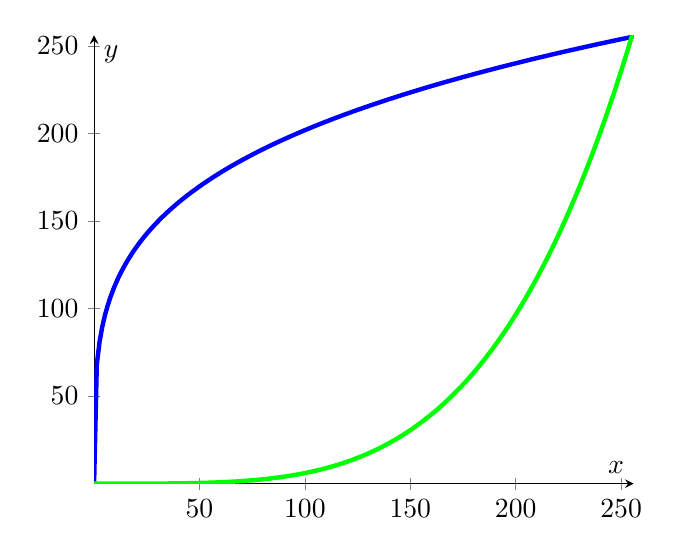
\begin{tikzpicture}[scale=01.0]
        \begin{axis}[
            axis x line=middle,
            axis y line=middle,
            ymin=0,ymax=256,ylabel=$y$,
            xmin=0,xmax=256,xlabel=$x$
            ]
        \addplot[domain=0:256, blue, ultra thick, samples=200] {255*(x/255)^0.25};
        \addplot[domain=0:256, green, ultra thick, samples=200] {255*(x/255)^4.0};
    \end{axis}
    \end{tikzpicture}
\caption{Graph of gamma function $(L-1)\left(\frac{r}{L-1}\right)^\gamma$ where $\gamma = 4$ (green) and $\gamma = \frac{1}{4}$ (blue).}
\label{fig:gamma}
\end{figure}

\begin{exmp}
    Contrast-enhancement: $T: r \mapsto c + c\sin\left(\frac{\pi(r-c)}{2c}\right)$ where $c = \frac{L - 1}{2}$. When $\gamma > 1$ the image is darkened, when $\gamma < 1$ the image is brightened, and when $\gamma = 1$ the image is unchanged.
\end{exmp}

\begin{figure}[ht!]
    \centering
    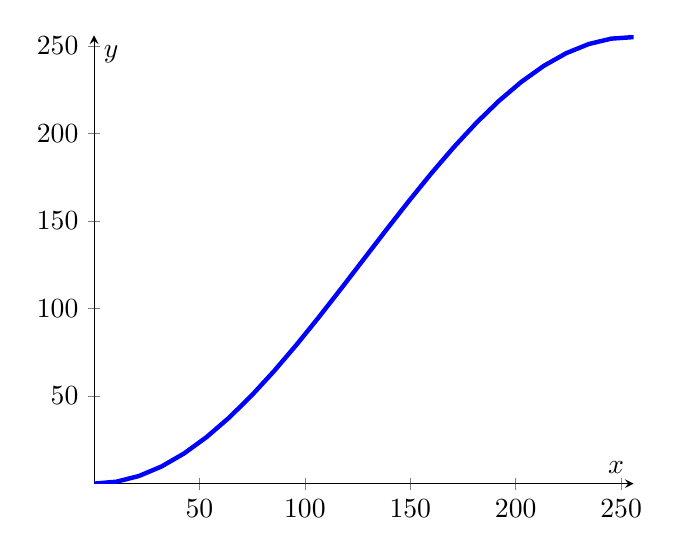
\begin{tikzpicture}[scale=01.0]
        \begin{axis}[
            axis x line=middle,
            axis y line=middle,
            ymin=0,ymax=256,ylabel=$y$,
            xmin=0,xmax=256,xlabel=$x$
            ]
        \addplot[domain=0:256, blue, ultra thick] {127.5 + 127.5*sin(deg(0.5*pi*(x - 127.5)/127.5))};
    \end{axis}
    \end{tikzpicture}
\caption{Graph of contrast enhancement $c + c\sin\left(\frac{\pi(r-c)}{2c}\right)$.}
\label{fig:contrast}
\end{figure}

\end{document}


\end{document}
